\documentclass[12pt, a4paper, reqno]{amsart}
\usepackage[slovene]{babel}
\usepackage[T1]{fontenc}
\usepackage[utf8]{inputenc}
\usepackage{amsmath,amssymb,amsfonts,amsthm}
\usepackage{url}
\usepackage[dvipsnames,usenames]{color}
\usepackage{graphicx}
\usepackage{tikz}
\usepackage{dsfont}
\usepackage{caption}
\usepackage{subcaption}
\usepackage{bm}
\usepackage{float}
\usepackage{xcolor}
\usepackage{bbm}
\usepackage{xcolor}
\usepackage[
    colorlinks=true,
    linkcolor=teal,      
    citecolor=teal,    
    filecolor=magenta,      
    urlcolor=cyan,   
]{hyperref}
%\usepackage{titlesec}
\allowdisplaybreaks

%--------------------------------------OBLIKA DOKUMENTA--------------------------------------------%

% Oblika strani
\textwidth 15cm
\textheight 24cm
\oddsidemargin.5cm
\evensidemargin.5cm
\topmargin-5mm
\addtolength{\footskip}{10pt}
\pagestyle{plain}
\overfullrule=15pt % oznaci predlogo vrstico

% Naslovi
%\titleformat{\section}
%{\normalfont\Large\bfseries\centering\MakeUppercase}{\thesection}{1em}{}
%
%\titleformat{\subsection}
%{\normalfont\large\bfseries}{\thesubsection}{1em}{}
%
%\titleformat{\subsubsection}
%{\normalfont\normalsize\bfseries}{\thesubsubsection}{1em}{}


% Matematicna okolja (tekst napisan pokoncno)
\theoremstyle{definition}
\newtheorem{definicija}{Definicija}[section]
\newtheorem{zgled}[definicija]{Zgled}
\newtheorem{opomba}[definicija]{Opomba}

\renewcommand\endzgled{\hfill$\diamondsuit$}

% Matematicna okolja (tekst napisan posevno)
\theoremstyle{plain} 
\newtheorem{lema}[definicija]{Lema}
\newtheorem{izrek}[definicija]{Izrek}
\newtheorem{trditev}[definicija]{Trditev}
\newtheorem{posledica}[definicija]{Posledica}



% Ukaz za slovarsko geslo
\newlength{\odstavek}
\setlength{\odstavek}{\parindent}
\newcommand{\geslo}[2]{\noindent\textbf{#1}\hspace*{3mm}\hangindent=\parindent\hangafter=1 #2}

% Podatki o delu
\newcommand{\program}{Finančna matematika} 
\newcommand{\imeavtorja}{Anej Rozman} 
\newcommand{\imementorja}{~doc.~dr. Martin Raič} 
\newcommand{\naslovdela}{Sestavljeni Poissonov proces in njegova uporaba v financah} 
\newcommand{\letnica}{2024} 

% Dodatni ukazi
\newcommand{\R}{\mathbb{R}}
\newcommand{\N}{\mathbb{N}}
\newcommand{\E}{\mathbb{E}}
\newcommand{\F}{\mathcal{F}}
\newcommand{\B}{\mathcal{B}}
\newcommand{\Prob}{\mathbb{P}}
\newcommand{\1}{\mathds{1}}
\newcommand{\Pois}[1]{\text{Pois}(#1)}
\newcommand{\Var}[1]{\text{Var}\left[#1\right]}

%------------------------------------------NASLOVNE STRANI-----------------------------------------%

\begin{document}

\thispagestyle{empty}
\noindent{\large
UNIVERZA V LJUBLJANI\\[1mm]
FAKULTETA ZA MATEMATIKO IN FIZIKO\\[5mm]
\program\ -- 1.~stopnja}
\vfill

\begin{center}{\large
\imeavtorja\\[2mm]
{\bf \naslovdela}\\[10mm]
Delo diplomskega seminarja\\[1cm]
Mentor: \imementorja}
\end{center}
\vfill

\noindent{\large
Ljubljana, \letnica}
\pagebreak

\thispagestyle{empty}
\tableofcontents
\pagebreak

\thispagestyle{empty}
\begin{center}
{\bf \naslovdela}\\[3mm]
{\sc Povzetek}
\end{center}

%--------------------------------------POVZETEK V SLOVENSCINI--------------------------------------%



%--------------------------------------------------------------------------------------------------%

\vfill
\begin{center}
{\bf Compound Poisson process and its application in finance}\\[3mm] 
{\sc Abstract}
\end{center}

%--------------------------------------POVZETEK V ANGLESCINI---------------------------------------%



%--------------------------------------------------------------------------------------------------%

\vfill\noindent
{\bf Math. Subj. Class. (2020):} 60G07 60G20 60G51 \\[1mm]
{\bf Klju"cne besede:} slu"cajni procesi, sestavljeni Poissonov proces,\newline Cramér--Lundbergov model\\[1mm]
{\bf Keywords:} stochastic processes, compound Poisson process, Cramér--Lundberg model
\pagebreak


%--------------------------------------------ZAHVALA-----------------------------------------------%
\addtocontents{toc}{\protect\setcounter{tocdepth}{0}}
\section*{Zahvala}
%Zahvaljujem se doc. dr. Martinu Rai"cu za njegovo mentorstvo. S širokim znanjem in izkušnjami 
%me je pomagal pri razumevanju in nadgradnji tematik, ki jih obravnavamo na dodiplomskem 
%"sutidiju Finan"cne matematike. Hvaležen sem mu za njegovo izjemno pripravljenost, za pomoč,
%večkratne diskusije, svetovanje pri dokazovanju izrekov in oblikovanju besedila, natančnost pri 
%pregledovanju napisanega teksta ter vzpodbude pri premagovanju ovir.
%
%Hvala tudi moji družini in prijateljem za podporo in spodbudo pri delu na tem diplomskem seminarju.
\addtocontents{toc}{\protect\setcounter{tocdepth}{2}}
\pagebreak
%--------------------------------------------VSEBINA-----------------------------------------------%

\section{Uvod}

    \begin{center}
        \framebox[\linewidth]{%
    \rule{0pt}{50pt}%
    Uvodni tekst in motivacija za "studiranje procesa, naka"zi da bo"s obravnaval Cramer-Ludenbergov model%
        }
    \end{center}

    \begin{figure}[H]
        \centering
        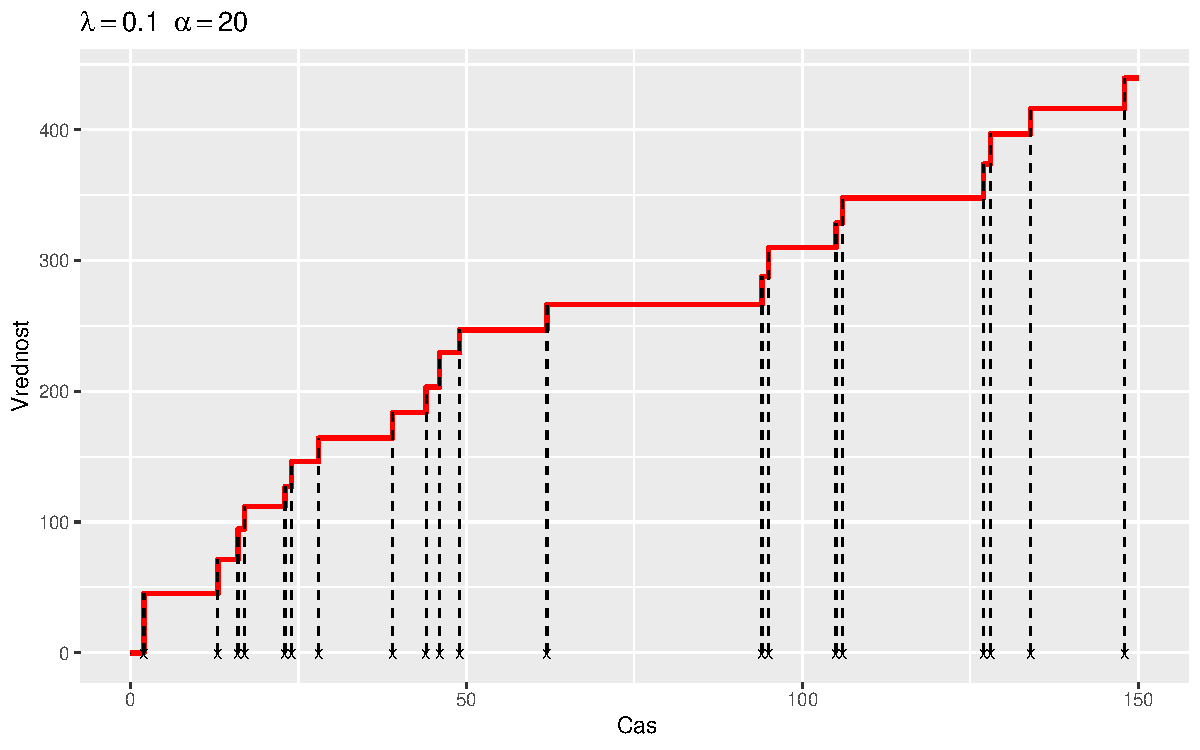
\includegraphics[width=\textwidth]{
            C:/Users/38651/OneDrive - Univerza v Ljubljani/Desktop/Diploma/Diplomski-seminar/GraphsAndPhotos/slika1.pdf
            }
        \caption{Primer trajektorije sestavljenega Poissonovega procesa}
        \label{fig:slika1}
    \end{figure}
    
    \noindent


    \begin{definicija}
        Naj bo $(\Omega, \mathcal{F}, \mathbb{P})$ verjetnostni prostor in naj bo $T\neq\emptyset$
        neprazna indeksna množica ter $(E, \Sigma)$ merljiv prostor. \textit{Slučajni proces}, 
        parametriziran s $T$, je družina slučajnih elementov $X_t : \Omega \to E$,
         ki so $(\mathcal{F}, \Sigma)$-merljivi za vsak $t \in T$.
        \label{def:slucProc}
    \end{definicija}

    \begin{opomba}
        V delu se bomo omejili na primer, ko $T$ predstavlja "cas, torej $T = [0, \infty)$ in da slu"cajne
        spremenljivke 
        zavzemajo vrednosti v realnih "stevilih, torej $(E, \Sigma) = (\R, \B_{\R})$, kjer $\B_\R$ 
        predstavlja Borelovo $\sigma-$algebro na $\R$.
        \label{op:Konvencije}
    \end{opomba}


    \begin{definicija}
        Za fiksen $\omega \in \Omega$ je preslikava 
        $[0, \infty) \rightarrow \mathbb{R}; \ t \mapsto X_t(\omega)$ 
        \textit{trajektorija} oziroma \textit{realizacija} slučajnega procesa $(X_t)_{t\geq0}$.
        Tako lahko slu"cajni proces gledamo kot predpis, ki vsakemu elementu vzor"cnega prostora 
        $\Omega$ priredi slu"cajno funkcijo
        $(X_t(\omega))_{t\geq0}: [0, \infty) \rightarrow \mathbb{R}$.
        \label{def:realizac}
    \end{definicija}

    \begin{definicija}
        Naj bo $(X_t)_{t\geq0}$ slu"cajni proces. Potem za $s < t$ definiramo
        \textit{prirastek procesa} $X_t - X_s$ na intervalu $[s, t]$. Proces $(X_t)_{t\geq0}$ ima 
        \textit{neodvisne prirastke}, če so za vsak nabor realnih "stevil
        $0 \leq t_1 < t_2 < \ldots < t_n < \infty$ prirastki
        $$
            X_{t_2} - X_{t_1}, \ X_{t_3} - X_{t_2}, \ \ldots, \ X_{t_n} - X_{t_{n-1}}
        $$
        med seboj neodvisni.
        \label{def:prirastek}
    \end{definicija}

    \begin{definicija}
        Naj bo $(X_t)_{t\geq0}$ slu"cajni proces. Potem pravimo, da ima proces
        \textit{stacionarne prirastke}, "ce za vsak $s < t$ in vsak $h > 0$ velja, 
        da ima $X_{t+h} - X_{s+h}$ enako porazdelitev kot $X_t - X_s$.
        \label{def:stacPrir}
    \end{definicija}

    \begin{definicija}
        Naj bo $\lambda > 0$. Slučajnemu procesu $(N_t)_{t\geq 0}$, definiranem na verjetnostnem 
        prostoru $(\Omega, \mathcal{F}, \mathbb{P})$ z vrednostmi v $\N_0$, pravimo 
        \textit{Poissonov proces} z intenzivnostjo $\lambda$, če zadošča naslednjim pogojem:
        \begin{enumerate}
            \item $N_0 = 0$ \ $\Prob$-skoraj gotovo.
            \item $(N_t)_{t\geq 0}$ ima neodvisne in stacionarne prirastke,
            \item Za $0 \leq s < t$ velja $ N_t - N_s \sim\Pois{\lambda(t - s)}$,
        \end{enumerate}
        \label{def:HPP}
    \end{definicija}
\textcolor{red}{
    \begin{opomba}
        Vidimo, da v definiciji ne zahtevamo, da so skoki procesa le +1. To sledi iz...
        \label{op:skoki}
    \end{opomba}
}

\section{Sestavljena Poissonova porazdelitev}

    \begin{definicija}
        Naj bo $N\sim \Pois{\lambda}$  za $\lambda >0$ in $X_1, X_2, \dots$ zaporedje neodvisnih
        enako porazdeljenih slučajnih spremenljivk. Potem ima slu"cajna spremenljivka $S$ \textit{sestavljeno
        Poissonovo porazdelitev} "ce je njena porazdelitev enaka porazdelitvi slu"cajne spremenljivke
        \begin{equation*}
            S = \sum_{i=1}^NX_i,
        \end{equation*}
    \end{definicija}

    \begin{trditev}
        Naj bo $(X_t)_{t\geq0}$ slu"cajni proces na $(\Omega, \F, \mathbb{P})$. Potem ima $(X_t)_{t\geq0}$
        neodvisne prirastke natanko tedaj, ko je za vsak nabor realnih "stevil 
        $0 \leq t_1 < \ldots < t_n < t_{n+1} <\infty$ prirastek $X_{t_{n+1}} - X_{t_n}$ neodvisen od
        slu"cajnega vektorja $(X_{t_1}, \dots, X_{t_n})$.
        \label{trd:ekvivKarakterizacija}
    \end{trditev}

    \begin{proof}
        $(\Rightarrow):$

        $(\Leftarrow):$
    \end{proof}

    \begin{trditev}
        Naj bo $N\sim \Pois{\lambda}$  za $\lambda >0$ in $X_1, X_2, \dots X_n$ neodvisne s.s. (neodvisne 
        med sabo in od $N$) enako porazdeljene kot
        $$ X\sim
        \begin{pmatrix}
            a_1 & a_2 & a_3  \dots & \\
            \tfrac{\lambda_1}{\lambda} & \tfrac{\lambda_2}{\lambda} & \tfrac{\lambda_3}{\lambda} \dots & 
        \end{pmatrix},
        $$
        za poljubne $a_1, a_2, \dots, a_n \in \R$ in 
        $\lambda_1, \lambda_2, \dots, \lambda_n \in \R^+$ za katere velja 
        ${\sum_{i=1}^n\lambda_i = \lambda}$.
        Potem velja 
        \begin{equation*}
            \sum_{j=1}^\infty a_jY_j \sim \sum_{j=1}^NX_j,
        \end{equation*}
        kjer so $Y_1,Y_2,  \dots$ neodvisne s.s.\ porazdeljene kot 
        $\Pois{\lambda_1},\Pois{\lambda_2}, \dots$
        \label{trd:NXjeEnakoaY}
    \end{trditev}

    \begin{proof}
        S $\varphi_{Z_n}(u)$ ozna"cimo karakteristi"cno funkcijo s.s.\ 
        $Z_n := a_1Y_1 + a_2Y_2 + \dots + a_nY_n$ in s $\varphi_{Z}(u)$ karakteristi"cno funkcijo s.s.\
        $Z:= \sum_{j=1}^{N}X_j$. Po neodvisnosti velja
        \begin{align*}
            \varphi_{Z_n}(u) 
                    &= \prod_{j=1}^{n}\varphi_{Y_j}(a_ju)\\
                    &= \prod_{j=1}^{n}\exp\left[\lambda_j\left(e^{a_j i u} - 1\right)\right] \\
                    &= \exp\left[\sum_{j=1}^{n}\lambda_j\left(e^{a_j i u} - 1\right)\right].
        \end{align*}

        \noindent
        Po trditvi \ref{trd:povezavaRodovneKarkateristicne} velja
        \begin{align*}
            \varphi_{Z}(u) 
                    &= G_N\left(\varphi_X(u)\right) \\
                    &= \exp\left[\lambda\left(\varphi_X(u) - 1\right)\right] \\
                    & = \exp\left[\lambda\left(\sum_{j=1}^\infty\frac{\lambda_j}{\lambda}e^{a_jiu} - 1\right)\right]\\
                    &= \exp\left[\sum_{j=1}^{\infty}\lambda_j\left(e^{a_j i u} - 1\right)\right]
        \end{align*}

        \noindent 
        Vidimo, da velja%Rezultat je posledica inverzne formule za karateristi"cne funkcije.
        \begin{equation*}
            \varphi_{Z_n} \xrightarrow{n\to\infty}\varphi_Z,
        \end{equation*}
        torej po Lévijevem izreku o kontinuiteti velja $Z_\infty :=\lim_{n\to\infty}Z_n \sim Z$.
    \end{proof}

    \begin{posledica}
        Naj bo $(a_n)_{n\in\N}$ poljubno zaporedje realnih "stevil in $(\lambda_n)_{n\in\N}$ zaporedje 
        pozitivnih realnih "stevil, za katere velja $\sum_{n=1}^\infty\lambda_n = \lambda$ in 
        \begin{equation*}
            X\sim
            \begin{pmatrix}
                a_1 & a_2 &  \dots \\
                \tfrac{\lambda_1}{\lambda} & \tfrac{\lambda_2}{\lambda} & \dots
            \end{pmatrix}.
        \end{equation*}
        Potem velja
        \begin{equation*}
            \sum_{j=1}^{n}a_jY_j \xrightarrow[n\to\infty]{d}\sum_{j=1}^NX_j,
        \end{equation*}
        \label{pos:NXjeEnakoaYstevno}
    \end{posledica}

    \begin{proof}
        Ker velja $\varphi_{Z_n}(u) \xrightarrow{n\to\infty} \varphi_{Z}(u)$ za vsak $u\in\R$, po Lévijevem
        izreku o zveznosti sledi, da $Z_n \xrightarrow[n\to\infty]{d} Z$.
    \end{proof}

    Kaj pa v primeru, ko so $X_i$ zvezno porazdeljene? 
    Tedaj se problema lotimo na slede"c na"cin. Definiramo $F_n(x) := F(\tfrac{m}{n})$ kjer je
    $F(x)$ porazdelitvena funkcija slu"cajne spremenljivke $Z_n$ in 
    $m = \min\{k \in \mathbb{Z} \mid \tfrac{k}{n} > F_n(x)\}$.

        \begin{figure}[H]
            \begin{center}
            
                \begin{tikzpicture}
                    % coordinate system
                    \draw[->] (-0.75,0) -- (9,0) node[right] {$x$};
                    \draw[->] (2,0) -- (2,4.5) node[above] {$F, F_n$};
                    \draw (2, 3.4) -- (2, 3.4) node[left] {$1$};
                    \draw[dashed] (-0.75,3.2) -- (9,3.2);
                
                    % CDF of continuous random variable
                    \draw[blue] (-0.75, 0.1) .. controls (0,0.2) and (2.2, 0.3) .. (2.8, 1.2);
                    \draw[->, blue] (2.8, 1.2) .. controls (3.1, 1.7) and (3.6, 2) .. (5, 2.1);
                    \filldraw[blue] (5, 2.5) circle (0.7pt);
                    \draw[blue] (5, 2.5) .. controls (6, 2.8) and (7.5, 3) .. (9, 3.15) node[below] {$F(x)$};
                
                    % CDF of F_n, 
                    \draw[->, red] (-0.75, 0.22) -- (0.25, 0.22);
                    \filldraw[red] (-0.75, 0.22) circle (0.7pt);
                    \draw[->, red] (0.25, 0.39) -- (1.25, 0.39);
                    \filldraw[red] (0.25, 0.39) circle (0.7pt);
                    \draw[->, red] (1.25, 0.74) -- (2.25, 0.74);
                    \filldraw[red] (1.25, 0.74) circle (0.7pt);
                    \draw[->, red] (2.25, 1.68) -- (3.25, 1.68);
                    \filldraw[red] (2.25, 1.68) circle (0.7pt);
                    \draw[->, red] (3.25, 2.01) -- (4.25, 2.01) node[above left]{$F_n(x)$};
                    \filldraw[red] (3.25, 2.01) circle (0.7pt);
                    \draw[->, red] (4.25, 2.58) -- (5.25, 2.58);
                    \filldraw[red] (4.25, 2.58) circle (0.7pt);
                    \draw[->, red] (5.25, 2.79) -- (6.25, 2.79);
                    \filldraw[red] (5.25, 2.79) circle (0.7pt);
                    \draw[->, red] (6.25, 2.94) -- (7.25, 2.94);
                    \filldraw[red] (6.25, 2.94) circle (0.7pt);
                    \draw[->, red] (7.25, 3.07) -- (8.25, 3.07);
                    \filldraw[red] (7.25, 3.07) circle (0.7pt);
                
                
                    %intervals of F_n
                
                \end{tikzpicture}
                \caption{Aproksimacija $F$ s $F_n$}
                \label{fig:slika2}
            \end{center}
        \end{figure}

    \noindent
    Kot je razvidno iz slike \ref{fig:slika2}, je $F_n(x)$ stopni"casta funkcija, ki aproksimira 
    porazdelitveno funkcijo $F(x)$. Velja $F_n \xrightarrow{n\to\infty}F$ povsod kjer je $F$ zvezna.


\section{Sestavljeni Poissonov proces}

    \begin{center}
        \framebox[\linewidth]{%
    \rule{0pt}{50pt}%
        Povzetek poglavja/krajsi uvod%
        }
    \end{center}
    \begin{definicija}
        Naj bo $(N_t)_{t\geq0}$ Poissonov proces z intenzivnostjo $\lambda$. 
        Naj bo $(X_i)_{i\geq1}$ zaporedje neodvisnih (med sabo in $(N_t)_{t\geq0}$) in enako 
        porazdeljenih slučajnih spremenljivk z vrednostmi v $\mathbb{R}$. Potem je 
        \textit{sestavljeni Poissonov proces} $(S_t)_{t\geq0}$ definiran kot
        $$
            S_t = \sum_{i=1}^{N_t} X_i.
        $$
        \label{def:CPP}
    \end{definicija}

    \begin{opomba}
        Vidimo, da je sestavljeni Poissonov proces posplo"sitev homogenega Poissonovega procesa, saj "ce za
        $X_i$ vzamemo konstantno funkcijo $X_i = 1$ za vsak $i$, dobimo ravno $HPP$. Bolj v splo"snem, "ce za $X_i$ 
        postavimo $X_i = \alpha$, potem velja $S_t = \alpha N_t$.
        \label{op:CPPHPPPovezava}
    \end{opomba}

    V nadaljevanju bomo homogen Poissonov proces z intenzivnostjo $\lambda >0$ ozna"cevali s $HPP(\lambda)$ 
    ali naborom slu"cajnih spremenljivk $(N_t)_{t\geq0}$ (angl. Homogeneous Poisson Process), 
    sestavljeni Poissonov proces pa s $CPP$ ali naborom slu"cajnih spremenljivk $(S_t)_{t\geq0}$ 
    (angl. Compound Poisson Process), kjer bo vsota sledila $HPP(\lambda)$.

    \subsection{Osnovne lastnosti}

        \begin{trditev}
            $CPP$ ima neodvisne in stacionarne prirastke.
            \label{trd:neodvPrirCPP}
        \end{trditev}

        \begin{proof}
            Za nabor realnih "stevil $0 \leq t_1 < t_2 < \ldots < t_n < \infty$ lahko slu"cajne
            spremeljivke $S_{t_i} - S_{t_{i-1}}$ zapi"semo kot
            \begin{align*}
                S_{t_i} - S_{t_{i-1}} &= \sum_{j=N_{t_{i-1}}+1}^{N_{t_i}} X_j. 
            \end{align*}
            Neodvisnost prirastkov sledi po neodvisnosti $X_i$ od $X_j$ za $i\neq j$ in $N_t$. 
            Naj bo $h > 0$ in $s < t$. Potem velja
            \begin{align*}
                S_{t+h} - S_{s+h} &= \sum_{j=N_{s+h}+1}^{N_{t+h}} X_j \\
            \end{align*}
            Vsota ima $N_{t+h} - N_{s+h}$ členov. Ker za $HPP$ velja 
            $N_{t+h} - N_{s+h} \sim N_t - N_s$, je 
            \begin{align*}
                \sum_{j=N_{s+h}+1}^{N_{t+h}} X_j = \sum_{j=N_{s}+1}^{N_{t}} X_j = S_t - S_s.
            \end{align*}
        \end{proof}

        \begin{trditev}
            Naj bo $(S_t)_{t\geq 0}$ $CPP$ in naj bosta $\mu = \E\left[X_i\right] < \infty$ 
            pri"cakovana vrednost in $\sigma^2= \Var{X_i} <\infty$ varianca
            slu"cajnih spremenljivk $X_i$ za vsak $i$. Potem sta za $t\geq0$ pri"cakovana vrednost in 
            varianca $S_t$ enaki 
            \begin{equation*}
                \E\left[S_t\right] = \mu\lambda t \qquad \text{in} \qquad \Var{S_t} = \lambda t\left(\sigma^2 + \mu^2\right).
            \end{equation*}
            \label{trd:PricVarCPP}
        \end{trditev}

        \begin{proof}

            Definiramo slu"cajno spremenljivko
            \begin{equation}
                Y_k = X_1 + X_2 + \cdots + X_k
                \label{eq:Y_k}
            \end{equation}
            in vidimo, da je za $t\geq0$ $S_t$ pogojno na $N_t = k$ enako porazdeljena 
            kot $Y_k$. Tako dobimo 
            \begin{align*}
            \E\left[S_t\mid N_t = k\right] = \E\left[Y_k\right] = k\mu \qquad \text{in} \qquad
            \Var{S_t\mid N_t = k} = \Var{Y_k} = k\sigma^2.
            \end{align*}
            Po formuli za popolno pri"cakovano vrednost velja 
            $\E\left[S_t\right] = \E\left[\E\left[S_t\mid N_t\right]\right]$. Torej

            \begin{align*}
                \E\left[S_t\right] = \E\left[\E\left[S_t\mid N_t\right]\right] = \E\left[\mu N_t\right] = \mu\lambda t.
            \end{align*}

            \noindent
            Prek formule $\Var{S_t} = \E\left[\Var{S_t\mid N_t}\right] + \Var{\E\left[S_t\mid N_t\right]}$ ra"cunamo 

            \begin{equation*}
                \E\left[\Var{S_t\mid N_t}\right] = \E\left[\Var{X_i}N_t\right] = \sigma^2\lambda t
            \end{equation*}
            in 
            \begin{equation*}
                \Var{\E\left[S_t\mid N_t\right]} = \Var{\E\left[X_i\right]N_t} = \mu^2\lambda t,
            \end{equation*}
            saj $N_t\sim\Pois{\lambda t}$. Skupaj dobimo $\Var{S_t} = \lambda t\left(\sigma^2 + \mu^2\right)$.
        \end{proof}

    \subsection{Rodovne funkcije}

    \begin{trditev}
        Naj bo $(S_t)_{t\geq0}$ $CPP$. Naj bodo slu"cajne spremenljivke $X_i$, ki jih se"stevamo v 
        $CPP$ enako porazdeljene kot $X$. Potem ima za $t\geq0$ karakteristi"cna funkcija $\varphi_{S_t}$ 
        obliko
        \begin{equation*}
            \varphi_{S_t}(u) = e^{\lambda t\left(\varphi_X(u) - 1\right)}, 
        \end{equation*}
        kjer $\varphi_X$ ozna"cuje karakteristi"cno funkcijo $X$.
        \label{trd:MomentGener}
    \end{trditev}
    
    \begin{proof}
        \begin{align}
            \varphi_{S_t}(u) 
                    &= \E\left[\exp\left[iuS_t\right]\right] = \nonumber
                        \E\left[\exp\left[iu\sum_{i = 1}^{N_t}X_i\right]\right] \nonumber\\
                    &= \sum_{k=0}^{\infty}
                        \E\left[\exp\left[iu\sum_{i = 1}^{N_t}X_i\mid N_t=k\right]\right]\Prob\left(N_t = k\right) \nonumber \\ 
                    &= \sum_{k=0}^{\infty}
                        \E\left[\exp\left[iu\sum_{i = 1}^kX_i\right]\right]\Prob\left(N_t = k\right) \nonumber \\
                    &= \sum_{k=0}^{\infty}
                        \underbrace{\E\left[e^{iuX}\right]^k}_{\varphi_X(u)^k}\frac{(\lambda t)^k}{k!}e^{-\lambda t} \label{eq:MomentS_t}\\ 
                    &= e^{-\lambda t} + e^{-\lambda t}\sum_{k=1}^\infty\frac{\left(\varphi_X(u)\lambda t\right)^k}{k!} \nonumber \\
                    &= e^{\lambda t\left(\varphi_X(u) - 1\right)} \nonumber
        \end{align}
    \end{proof}

    Hitro lahko vidimo, da sta karakteristi"cna in rodovna funkcija $CPP$ enaki

    \begin{equation*}
        \varphi_{S_t}(u) = e^{\lambda t\left(\varphi_X(u) - 1\right)} \qquad \text{in} \qquad 
        G_{S_t}(u) = e^{\lambda t\left(G_X(u) - 1\right)},
    \end{equation*} 

    \noindent
    saj v splo"snem velja, da je karakteristi"cna funkcija neke slu"cajne spremenljivke $Y$ enaka
    njeni momentno rodovni funkciji izvrednoteni v $iu$, torej $\varphi_Y(u) = G_Y(iu)$. Rodovna pa 
    izverdnotena v $\ln(u)$, torej $G_Y(u) = M_Y(\ln(u))$, "ce obstajata.
    V nadaljevanju bomo uporabljali predvsem karakteristi"cno funkcijo $CPP$, saj je ta vedno definirana 
    za vsak $u\in\R$. Prav nam bo pri"sla tudi naslednja povezava med karakteristi"cno funkcijo $CPP$ 
    in rodovno funkcijo $HPP(\lambda)$.
    \begin{trditev}
        Naj bosta $(S_t)_{t\geq0}$ $CPP$ in $(N_t)_{t\geq0}$ $HPP(\lambda)$ neodvisna. 
        Naj bodo slu"cajne spremenljivke $X_i$, ki jih se"stevamo v $CPP$ enako porazdeljene kot $X$. 
        Potem za fiksen $t\geq0$ velja

        \begin{align*}
            \varphi_{S_t}(u) = G_{N_t}\left(\varphi_{X}(u)\right).
        \end{align*}

        \label{trd:povezavaRodovneKarkateristicne}
    \end{trditev}

    \begin{proof}
        Po ena"cbi (\ref{eq:MomentS_t}) iz trditve \ref{trd:MomentGener} velja, da je $\varphi_{S_t}(u)$ enaka
        \begin{align*}
            \varphi_{S_t}(u) &= \sum_{k=0}^{\infty}
            \varphi_X(u)^n\frac{(\lambda t)^k}{k!}e^{-\lambda t} \\
            &= G_{N_t}\left(\varphi_X(u)\right).
        \end{align*}
    \end{proof}

    \subsection{Porazdelitev CPP}
    Sedaj se posvetimo vpra"sanju, kako je porazdeljena slu"cajna spremenljivka $S_t$ za $t\geq 0$? 
    Iz definicije $HPP(\lambda)$ vemo, da je $N_t$ za $t\geq0$ porazdeljena kot Poissonova slu"cajna 
    spremenljivka s parametrom $\lambda t$. Fiksiramo $t\geq0$ in dobimo 

    \begin{align*}
        F_{S_t}(x) = \Prob(S_t \leq x) 
        &= \sum_{k=0}^\infty \Prob(S_t \leq x \mid N_t = k)\Prob(N_t = k) \\
        & = \sum_{k=0}^\infty \Prob(\sum_{i=1}^k X_i \leq x)\frac{(\lambda t)^k}{k!}e^{-\lambda t} \\
        & = \sum_{k=0}^\infty F_X^{*k}(x)\frac{(\lambda t)^k}{k!}e^{-\lambda t}, \\
    \end{align*}

    \noindent
    kjer je $F_X^{*k}(x)$ porazdelitev $k$-te konvolucije slu"cajne spremenljivke $X$. Razen za 
    posebne primere, je zgornji izraz za prakti"cne namene ne-izra"cunljiv in nam ne pomaga veliko.
    
    \begin{zgled}
        "Ce pogledamo primer, ko so $X_1, X_2, \dots$ neodvisne enako porazdeljene slu"cajne spremenljivke,
        porazdeljene kot $X$
        \begin{equation*}
            X\sim\text{Exp}(a) \qquad \qquad f_X(x) = ae^{-ax}\mathbbm{1}_{(0, \infty)}(x),
        \end{equation*}
        s parametrom $a>0$, lahko pridemo do  eksplicitne porazdelitve $CPP$. Gostota $k$-te 
        konvolucije $X_1 + \cdots + X_k$ je porazdeljena kot $\text{Gamma}(k, a)$ in ima formulo
        \begin{equation*}
            f_{X_1 + \cdots + X_k}(x) = \frac{1}{\Gamma(k)}a^kx^{k-1}e^{-ax}\mathbbm{1}_{(0, \infty)}(x).
        \end{equation*}
        Za $t\geq 0$ in $x \geq 0$ torej velja
        \begin{align*}
            F_{S_t}(s) = \Prob(S_t \leq s)
            &= \sum_{k=0}^\infty \int_0^s\frac{1}{\Gamma(k)}a^ks^{k-1}e^{-as}ds\frac{(\lambda t)^k}{k!}e^{-\lambda t}
            \qquad \qquad \text{Tonelli} \ (\ref{izr:TonellijevIzrek}) \\
            &= \int_0^s\sum_{k=0}^\infty \frac{1}{\Gamma(k)}a^ks^{k-1}e^{-as}\frac{(\lambda t)^k}{k!}e^{-\lambda t}ds
        \end{align*}

        

    \end{zgled}
    
    %Poka"zimo, da je $CPP$ v resnici porazdeljen, kot limita linearne 
    %kombinacije neodvisnih Poissonovih slu"cajnih spremenljivk. 
    
    %\noindent
    %"Ce sedaj po"sljemo $n \to \infty$, dobimo
    %\begin{align}
    %    \varphi_{Z}(u) := \lim_{n\to\infty}\varphi_{Z_n}(u) = e^{\sum_{j=1}^{\infty}\lambda_j\left(e^{a_j i u} - 1\right)}.
    %    \label{eq:karFunkcVrste}
    %\end{align}
%
    %\noindent
    %Kot smo izpeljali zgoraj je karakteristi"cna funkcija $CPP$ podana s predpisom
%
    %\begin{align*}
    %    \varphi_{S_t}(u) = e^{\lambda t\left(\varphi_X(u) - 1\right)}, 
    %\end{align*}
%
    %\noindent
    %kar lahko zapi"semo kot 
%
    %\begin{align*}
    %    \varphi_{S_t}(u) = e^{\lambda t\int_{\R}\left(e^{i u z} - 1\right) \mu(dz)},
    %\end{align*}
%
    %\noindent
    %kjer je $\mu := X*\Prob$ potisk mere naprej po s.s.\ $X$. Prav tako lahko (\ref{eq:karFunkcVrste}) zapi"semo
    %kot 
%
    %\begin{align*}
    %    \varphi_{Z}(u) = e^{\int_{\R}\left(e^{i u x} - 1\right)\nu(dx)},
    %\end{align*}
%
    %\noindent
    %Za neko ustrezno mero $\nu$. Vidimo, da ko po"sljemo $n\to \infty$, za ustrezen izbor 
    %$a_1, a_2, \dots$ in $\lambda_1, \lambda_2, \dots$ karakteristi"cna funkcija 
    %vrste $Z_n$ konvergira h karakteristi"cni funkciji $S_t$. Torej po Lévijevem izreku o zveznosti 
    %sledi, da je $S_t$ enako porazdeljena kot $Z = \sum_{i=1}^{\infty}\alpha_iY_i$.
%

%    \subsection{CPP kot martingal}
%
%        \begin{definicija}
%            Slu"cajni proces $X_t$ prilagojen glede na filtracijo $(\F_t)_{t\geq0}$
%            martingal, "ce velja 
%            $$
%                \E\left[X_t\mid\F_s\right] = X_s
%            $$
%            za vsak $0\leq s \leq t$.
%            \label{def:martingal}
%        \end{definicija}
%
%        Poka"zimo, da v splo"snem $CPP$ ni martingal.
%
%        \begin{trditev}
%            Naj bo $(S_t)_{t\geq0}$ $CPP$ z intenzivnostjo $\lambda>0$ in naj bodo $X_i$ neodvisne
%            in enako porazdeljene slu"cajne spremenljivke z $\E\left[X_i\right] = \mu$ za vsak $i$.
%            Potem je $S_t$ martingal natanko tedaj, ko je $\mu = 0$.
%            \label{trd:CPPnimartingal}
%        \end{trditev}
%
%        \begin{proof}
%            Naj bo $0\leq s\leq t$. Potem velja
%            \begin{align*}
%                \E\left[S_t\mid\F_s\right] 
%                        &= \E\left[S_t - S_s + S_s\mid \F_s\right] \\
%                        &= \E\left[S_t - S_s\right] + \E\left[S_s\mid \F_s\right] \\
%                        &= \mu\lambda(t-s) + S_s
%            \end{align*}
%           Enakost $\mu\lambda(t-s) + S_s = S_s$ velja $\iff$ $\mu\lambda(t-s) = 0 \iff \mu = 0$.
%        \end{proof}
%
%        \begin{opomba}
%            Seveda, "ce velja $\mu \geq 0$, potem je $S_t$ submartingal, "ce pa $\mu \leq 0$, je
%            $S_t$ supermartingal.
%        \end{opomba}
%
%        \begin{trditev}
%            Naj bo $(S_t)_{t\geq0}$ CPP z intenzivnostjo $\lambda > 0$ in naj bodo $X_i$ neodvisne
%            in enako porazdeljene slu"cajne spremenljivke z $\E\left[X_i\right] = \mu$ za vsak $i$,
%            Potem je proces 
%            $$
%                S_t - \mu\lambda t
%            $$
%            martingal.
%            \label{trd:CPPpostanemartingal}
%        \end{trditev}
%
%        \begin{proof}
%            Naj bosta $0 \leq s < t$. Prirastek $S_t - S_s$ je neodvisen od $\F_s$ in ima 
%            pri"cakovano vrednost $\mu\lambda(t-s)$. Torej 
%            \begin{align*}
%                \E\left[S_t - \mu\lambda t\mid\F_s\right] 
%                        &= \E\left[S_t - S_s\right] + S_s - \mu\lambda t\\
%                        &= \mu\lambda(t-s) + S_s - \mu\lambda t\\
%                        &= S_s - \mu\lambda s.
%            \end{align*}
%        \end{proof}
%
%        %\subsection{"Cas prvega prehoda}
%        %Postavimo si vpra"sanje, kdaj bo $CPP$ prvi"c dosegel nek $a\in\R$. Obravnavajmo primer, ko je 
%        %$a>0$, saj je primer, ko je $a$ negativen simetri"cen. Naj bo $T_a = \inf\{t\geq0; S_t \geq a\}$ 
%        %"cas prvega prehoda $CPP$. V tem poglavju bomo izra"cunali porazdelitev $T_a$.
%        %"Ce pogledamo dogodek $\{T_a \leq t\}$.

    \subsection{Neskon"cna deljivost}

    \begin{definicija}
        Naj bo $X$ slu"cajna spremenljivka. Pravimo, da je $X$ \textit{neskon"cno deljiva}, "ce za vsak $n\in\N$
        obstajajo neodvisne slu"cajne spremenljivke $X_1, X_2, \dots, X_n$ tako, da velja
        \begin{equation*}
            X \sim X_1 + X_2 + \cdots + X_n.
        \end{equation*}
        Ekvivalento lahko definiramo neskon"cno deljivost prek karakteristi"cne funkcije. Pravimo, da je
        slu"cajna spremenljivka $X$ neskon"cno deljiva, "ce je za vsak $n\in\N$ funkcija 
        $\left(\varphi_X(u)\right)^{\frac{1}{n}}$ karakteristi"cna funkcija neke slu"cajne spremenljivke.
    \end{definicija}

    \begin{zgled}
        Naj bo $X\sim \text{Pois}(\lambda)$. Potem je $X$ neskon"cno deljiva. To neposredno sledi 
        iz dejstva, da je karakteristi"cna funkcija vsote n.e.p.\ s.s.\ enaka produktu karateristi"cnih 
        funkcij, torej za $n\in\N$ in $u\in\R$ velja $\varphi_{X_1 + X_2 + \cdots + X_n}(u) = \varphi_X(u)^n$. 
        "Ce vzamemo $X_i \sim \text{Pois}(\tfrac{\lambda}{n})$, potem je 
        \begin{equation*}
        \varphi_{X_1 + X_2 + \cdots + X_n}(u) = 
        \left(\varphi_{X_i}(u)\right)^n = \left(e^{\tfrac{\lambda}{n}(e^{iu} - 1)}\right)^n = e^{\lambda(e^{iu} - 1)} = \varphi_X(u).
        \end{equation*}
    \end{zgled}

    Sedaj poka"zimo, da je sestavljena Poissonova porazdelitev neskon"cno deljiva, "se ve"c, poka"zimo, 
    da "ce je $S$ neskon"cno deljiva slu"cajna spremenljivka in zavzema vrednosti v $\N_0$, 
    potem ima sestavljeno Poissonovo porazdelitev.

    \begin{trditev}
        Naj bo $S$ slu"cajna spremenljivka, porazdeljena sestavljeno Poissonovo s parametrom $\lambda > 0$.
        Potem je $S$ neskon"cno deljiva.
        \label{trd:CPDneskoncnoDeljiva}
    \end{trditev}

    \begin{proof}
        Zapi"simo $S = \sum_{i=1}^NX_i$, kjer so $X_i$ neodvisne in enako porazdeljene slu"cajne 
        spremenjivke s skupno karakteristi"cno funkcijo $\varphi_X(u)$ in $N\sim\Pois{\lambda}$. Iz 
        trditve \ref{trd:MomentGener} vemo, da je karakteristi"cna funkcija $S$ za $u\in \R$ enaka
        \begin{equation*}
            \varphi_S(u) = \varphi_N\left(\varphi_X(u)\right) = e^{\lambda\left(\varphi_X(u) - 1\right)}.
        \end{equation*}
        Potem za $n\in\N$ velja
        \begin{equation*}
            \varphi_{S}(u) = \left(e^{\frac{\lambda}{n}\left(\varphi_X(u) - 1\right)}\right)^n
        \end{equation*}
        in vidimo, da je fukcija $u\mapsto e^{\frac{\lambda}{n}\left(\varphi_X(u) - 1\right)}$ karakteristi"cna
        funckija slu"cajne spremenljivke $S_i = \sum_{i = 1}^MX_i$ kjer je $M\sim\Pois{\tfrac{\lambda}{n}}$.
    \end{proof}

    \begin{trditev}
        Naj bo $S$ slu"cajna spremenljivka, ki zavzame vrednosti v $\N_0$ in je neskon"cno deljiva.
        Potem ima $S$ sestavljeno Poissonovo porazdelitev.
        \label{trd:neskoncnoDeljivaYslediCPD}
    \end{trditev}

    \begin{proof}
        Ozna"cimo rodovno funkcijo $S$ z 
        \begin{equation*}
            G_S(u) = \sum_{k = 0}^\infty \underbrace{\Prob\left(S = k\right)}_{p_k}u^k.
        \end{equation*} 
        Pokazali bomo, da je $G_S(u)$ enaka rodovni funkciji neke slu"cajne spremenljivke, ki ima sestavljeno
        Poissonovo porazdelitev. Ker za nenegativne celo"stevilske slu"cajne spremenljivke velja 
        $\Prob\left(S = k\right) = \frac{G_S^{(k)}(0)}{k!}$, bo to pomenilo, da je $S$ sestavljeno Poissonova, 
        saj v tem primeru rodovna funkcija dolo"ca porazdelitev $S$.
        Ker je $S$ neskon"cno deljiva potem je za vsak $n\in\N$ 

        \begin{equation*}
            G_{S_n}(u) := \left(G_S(u)\right)^{\frac{1}{n}} = 
            \sum_{k = 0}^\infty\underbrace{\Prob\left(S_n = k\right)}_{p_{k_n}}u^k
        \end{equation*}
        rodovna funkcija neke slu"cajne spremenljivke $S_n$ in za vsak $u\in\R$ velja enakost
        \begin{equation*}
            G_{S_n}(u) = \left(G_{S_1}(u)\right)^n \ \text{oziroma} \ 
            \sum_{k = 0}^\infty p_{k}u^k = \left(\sum_{k = 0}^\infty p_{k_n}u^k\right)^n.
        \end{equation*}
        "Ce raz"sirimo desno stran ena"ce in predpostavimo $p_0 = 0$, dobimo, da bmora biti 
        $p_{0_n} = 0$ in posledi"cno tudi $p_1 = p_2 = \cdots = p_{n-1} = 0$. Ker to velja za poljuben 
        $n\in\N$ dobimo, da je $G_S(u) = 0$, kar pa je protislovje. Torej $p_0 > 0$ in zagotovo 
        $G_S(u) > 0$ za $u\in[0, 1]$. Velja $\lim_{n\to\infty}\left(\frac{G_S(u)}{p_0}\right)^{\frac{1}{n}} = 1$ za $t\in[0, 1]$.
        Velja $\lim_{x \to 0}\frac{\ln(1 + x)}{x} = 1.$
        \begin{equation*}
            \ln\left(\left(\frac{G_S(u)}{p_0}\right)^{\frac{1}{n}}\right) = \ln\left( 1 + \left(\left(\frac{G_S(u)}{p_0}\right)^{\frac{1}{n}} - 1\right)\right)
            \approx \left(\frac{G_S(u)}{p_0}\right)^{\frac{1}{n}} - 1 \ \text{ko} \ n\to\infty.
        \end{equation*}
        Za $u = 1$ dobimo
        \begin{equation*}
            \ln\left(\left(\frac{1}{p_0}\right)^{\frac{1}{n}}\right) \approx \left(\frac{1}{p_0}\right)^{\frac{1}{p_0}} - 1 \ \text{ko} \ n\to\infty.
        \end{equation*}



        

    \end{proof}

    Sedaj trditev \ref{trd:neskoncnoDeljivaYslediCPD} nadgradimo\dots

    \begin{trditev}
        Naj ima slu"cajna spremenljivka $S$ neskon"cno deljivo porazdelitev. Potem lahko $S$ zapi"semo
        izrazimo kot limito slu"cajni spremenljivk, ki imajo sestavljeno Poissonovo porazdelitev.
    \end{trditev}
\pagebreak

\section{Cramér-Lundbergov model}
    \noindent
    Razdelek je prirejen po \cite{3}, \cite{4} in  \cite{5}.

    V tem razdelku obravnavamo najbolj intenzivno raziskan model v teoriji propada, običajno imenovan 
    Cramér-Lundbergov model. V svoji najosnovnejši obliki 
    ga je v zgodnjih 1900. letih izpeljal "svedski aktuar Filip Lundberg, da bi ocenil ranljivost 
    zavarovalnice za propad. Čeprav je model v svoji ideji dokaj preprost, 
     zajema bistvo povezave ravni rezerv zavarovalnice in njene izpostavljenosti tveganju, 
    kar je razlog, zakaj je postal temeljni merilni model v teoriji propada.
    V preteklem stoletju je bilo razvitih veliko tehnik za analizo Cramér-Lundbergovega modela, 
    ki so se večinoma osredotočale na kvantifikacijo verjetnosti propada. V razdelku podamo 
    pregled glavnih rezultatov in osnovnih tehnik, ter jih ponazorimo na primerih, ko 
    zavarovalni"ske zahtevke modeliramo z lahkorepimi in te"zkorepimi porazdelitvami.

    \subsection{Proces tveganja in verjetnost propada}

        \begin{definicija}
            Naj bo $(S_t)_{t\geq0 }$ $CPP$, kjer so slu"cajne spremenljivke $(X_i)_{i\in\N}$, 
            ki jih se"stevamo s.g.\ nenegativne.\ \textit{Proces tveganja} v Cramér-Lundbergovem 
            modelu definiramo kot
            \begin{align*}
                U_t = u + p(t) - S_t,
            \end{align*}
            kjer je $u \geq 0$ za"cetni kapital zavarovalnice in $p(t)$ funkcija prihodkov iz premij. 
            \label{def:procesTveganja}
        \end{definicija}

        \begin{opomba}
            V resnici lahko veliko lastnosti procesa tveganja izpeljemo brez da predpostavimo, da prihodi 
            zahtevkov v $(S_t)_{t\geq0}$ sledijo homogenem Poissonovemu procesu,
            ampak splo"snem prenovitvenemu procesu (\ref{def:PrenovitveniProces}) in
            zato na za"cetku ne bomo uporabljali rezultatov, ki smo jih do sedaj v delu izpeljali.
            \label{op:procesTveganja}
        \end{opomba}

        Vrednost $U_t$ predstavlja kapital zavarovalnice ob "casu $t\geq0$. Standardno je za $p(t)$ 
        vzeti deterministi"cno funkcijo $p(t) = ct$, kjer je $c>0$ stopnja prihodkov premij.
        Uporaba linearne funkcije za modeliranje premijskega dohodka v Cramér-Lundbergovem 
        modelu ponuja realističen približek zato, ker zavarovalnice pogosto doživljajo 
        stabilno povečevanje premijskega dohodka skozi čas. Poleg tega je izbira linearne 
        funkcije preprosta, zato bomo v nadaljevanju privzeli $p(t) = ct$. Poglejmo si 
        realizaciji procesa tveganja, ko so zahtevki $X_i$ porazdeljeni Weibullovo 
        (\ref{def:WeibullovaPorazdelitev}) z razli"cnimi parametri. 

        \begin{zgled}
            Naj bo $(U_t)_{t\geq0}$ proces tveganja v Cramér-Lundbergovem modelu z za"cetnim kapitalom
            $u = 1000$ in $p(t) = 200t$ ter intenzivnostjo prihodov zahtevkov $\lambda=1$. % v $CPP$. 
            Naj bodo v prvem primeru (rde"ca) 
            zahtevki porazdeljeni kot $X_i \sim \text{Weibull}(2, 434)$ in v drugem primeru (modra) kot
            $Y_i \sim \text{Weibull}(\tfrac{1}{4}, 16)$.
            
            \begin{figure}[H]
                \centering
                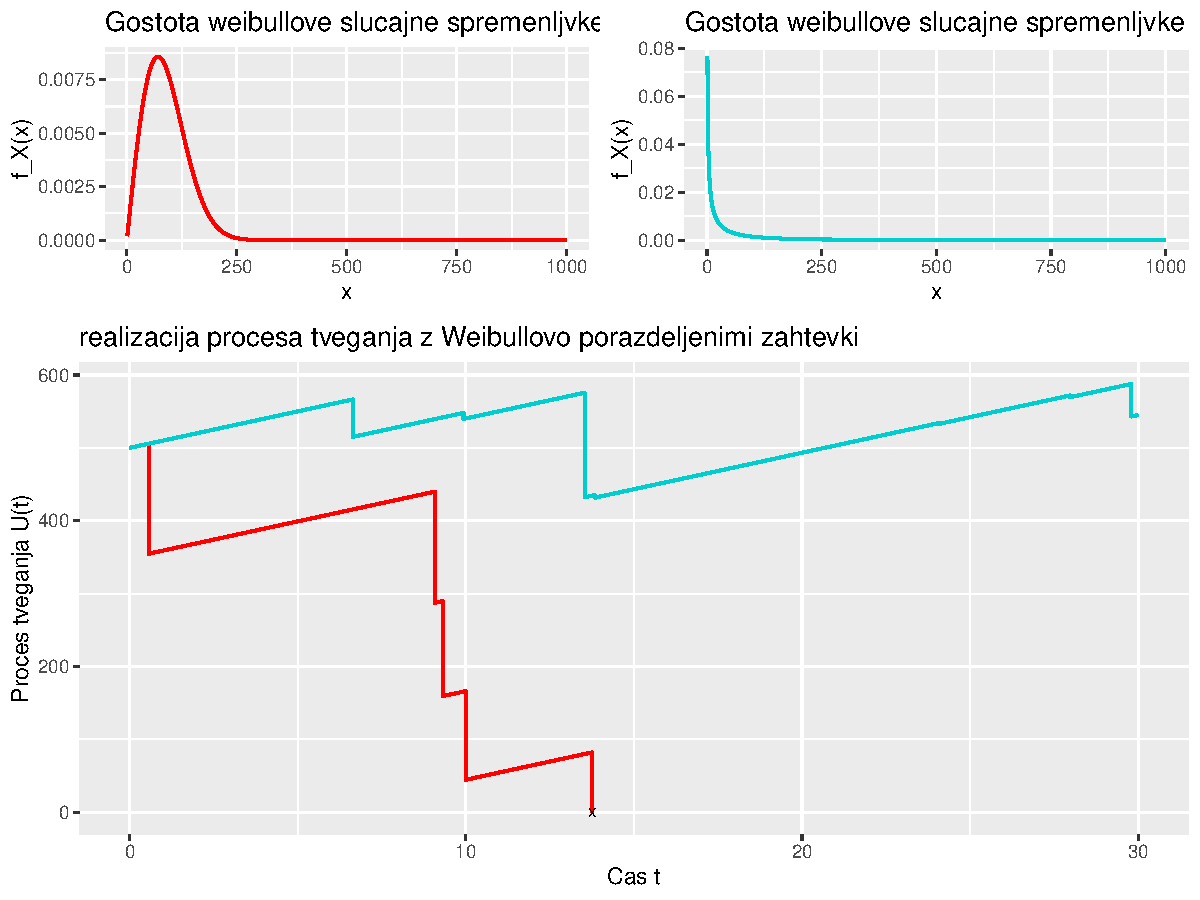
\includegraphics[width=\textwidth]{
                    C:/Users/38651/OneDrive - Univerza v Ljubljani/Desktop/Diploma/Diplomski-seminar/GraphsAndPhotos/slika2.pdf
                    }
                \caption{Realizaciji procesa tveganja}
                \label{fig:slika3}
            \end{figure}

            Pri obeh realizacijah vidimo, da proces tveganja v nekem trenutku pade pod $0$ (tam ga 
            tudi ustavimo). "Ceprav je pri"cakova vrednost 
            $\E\left[Y_i\right] = 384 \approx \E\left[X_i\right] = 217\sqrt{\pi} \approx 384,62$ 
            opazimo bistveno razliko med realizacijama. V rde"cem primeru proces pade pod
            $0$ po ve"c zaporednih manj"sih izgubah, v modrem primeru pa po eni zelo veliki izgubi. 
            V nadaljevanju bomo primera lo"cili, ampak pred tem 
            definirajmo osnovne pojme, ki jih bomo obravnavali v razdelku.

            \label{zgd:weibullProcesTveganja}
        \end{zgled}

        \begin{definicija}
            \textit{Propad} definiramo kot dogodek, da proces tveganja $(U_t)_{t\geq0}$ kadarkoli pade pod $0$. 
            Torej 
            \begin{align*}
                \bigl\{U_t<0 \ \text{za} \ t\geq 0\bigr\}
            \end{align*}
            in "casu ustavljanja
            \begin{align*}
                T = \inf\{t\geq0 \mid U_t < 0\}, 
            \end{align*}
            pravimo \textit{"cas propada}. Seveda velja enakost med dogodkoma
            \begin{align*}
                \{U_t<0 \ \text{za} \ t\geq0\} = \{T<\infty\}.
            \end{align*}
            \label{def:PropadCasPropada} 
        \end{definicija}

        \begin{definicija}
            \textit{Verjetnost propada} je definirana kot funckija $\psi(u): (0,\infty) \to [0,1]$ 
            podana s predpisom
            \begin{align*}
                \psi(u) = \Prob(T<\infty \mid U_0 = u).
            \end{align*}
            \label{def:VerjetnostPropada}
        \end{definicija}

        \begin{definicija}
            Po konstrukciji procesa tveganja $(U_t)_{t\geq0}$ je verjentost propada mogo"ca le ob 
            prihodih zahtevkov. %, ki sledijo $HPP(\lambda)$
            Z $V_n$ ozna"cimo "cas $n$-tega prihoda in definiramo 
            \textit{ogrodje procesa tveganja} kot $(U_{V_n})_{n\in\N}$.
            \label{def:ogrodjeProcesaTveganja}
        \end{definicija}

        \begin{trditev}
            Naj bo $(U_t)_{t\geq0}$ proces tveganja v Cramér-Lundbergovem modelu in $(U_{V_n})_{n\in\N}$ 
            njegovo ogrodje ter $T_n := V_n - V_{n-1}$ medpirhodni "cas $n$-tega zahtevka 
            $(V_0 = T_0 = 0)$. Potem velja 
            \begin{equation*}
                \psi(u) = \Prob\left(\sup_{n\in\N}Z_n > u\right),
            \end{equation*}
            kjer je $Z_n = \sum_{i=1}^nY_i$  komulativna izguba po $n$ prihodih in $Y_i = X_i - cT_i$
            izguba $i$-tega prihoda.
            \label{trd:verjetnostPropadaZOgrodjem}
        \end{trditev}

        \begin{proof}

            S pomo"cjo ogrodja procesa tveganja lahko dogodek propada zapi"semo kot
            \begin{align*}
                \bigl\{U_t<0 \ \text{za} \ t\geq 0\bigr\} &= 
                                \biggl\{\inf_{t\geq0}U_t<0\biggr\} \\
                              &= \biggl\{\inf_{n\in\N}U_{V_n}<0\biggr\} \\
                              &= \biggl\{\inf_{n\in\N}\bigl\{u + p(V_n) - S_{V_n}\bigr\} < 0\biggr\} \\
                              &= \biggl\{\inf_{n\in\N}\biggl\{u + 
                              \underbrace{cV_n - \sum_{i=1}^nX_i}_{-Z_n}\biggr\} < 0\biggr\} \\
                              &= \biggl\{\inf_{n\in\N}\{-Z_n\} < -u\biggr\} \\
                              &= \biggl\{\sup_{n\in\N}Z_n > u\biggr\},
            \end{align*}
            kar nam da "zeljeno enakost.
        \end{proof}

        Tako verjetnost propada prevedemo na prehodno verjetnost diskretnega slu"cajnega 
        sprehoda $(Z_n)_{n\in\N}$. V nadaljevanju nas bo predvsem zanimalo asimptoti"cno 
        vedenje $\psi(u)$, ko gre $u\rightarrow\infty$. Cilj obravnavanja verjetnosti propada v 
        Cramér-Lundbergovem modelu je, da se izognemo skoraj gotovemu propadu oziroma, da je verjetnost, da $(Z_n)_{n\in\N}$ prese"ze $u$
        tako majhna, da lahko v praksi dogodek propada izklju"cimo. 

        \begin{trditev}
            Naj bo $(Z_n)_{n\in\N}$ zaporedje slu"cajnih spremenljivk definirano kot 
            $Z_n = \sum_{i=1}^nY_i$ za neodvisne in enako porazdeljene slu"cajne spremenljivke 
            $Y_i$ z $\E\left[Y_i\right] < \infty$. Potem za vsak $u>0$ velja
            \begin{equation*}
                \Prob\left(\sup_{n\in\N}Z_n > u\right) = 1 \quad \text{za} \ u > 0,
            \end{equation*}
            "ce velja $\E\left[Y_i\right] \geq 0$.
            \label{trd:propadZVerjetnostjo1}
        \end{trditev}

        \begin{proof}
            Zaporedje slu"cajnih spremenljivk $(Y_i)_{i\in\N}$ zado"s"ca predpostavkam krepkega zakona
            velikih "stevil (\ref{izr:KrepkiZakonVelikihStevil}), torej velja
            \begin{equation*}
                \frac{Y_1 + Y_2 + \cdots Y_n}{n} = \frac{Z_n}{n} \xrightarrow[n\to\infty]{s.g.} \E\left[Y_n\right].
            \end{equation*}
            Torej bo $Z_n$ v primeru ko je $\E\left[Y_n\right]>0$
             skoraj gotovo asimptoti"cno linearno nara"scal proti $\infty$ kot $\E\left[Y_n\right] n$ in 
             bo za poljuben $u>0$
            \begin{equation*}
                \Prob\left(\sup_{n\in\N}Z_n > u\right) = 1.
            \end{equation*}
            Dokaz za primer, ko je $\E\left[Y_n\right] = 0$ je precej bolj tehni"cen in ne preve"c informativen, zato 
            ga bomo izpustili. Izka"ze se, da obstajata neki podzaporedji$(n_k)_{k\in\N}$ in $(m_k)_{k\in\N}$, da 
            $Z_{n_k} \xrightarrow[k\to\infty]{s.g.}\infty$ in 
            $Z_{m_k} \xrightarrow[k\to\infty]{s.g.}-\infty$.
            Dokaz lahko najdemo v \cite{6}.
        \end{proof}

        \begin{opomba}
            Iz trditve \ref{trd:propadZVerjetnostjo1} (ob predpostavkah $\E\left[X_i\right] < \infty$
            in $\E\left[T_i\right] < \infty$) sledi, da moramo premijo (in s tem $c$) izbrati tako, da bo 
            $\E\left[Y_i\right] < 0$, saj bo tako $Z_{n} \xrightarrow[n\to\infty]{s.g.}-\infty$
            in je to edini primer, ko lahko upamo, da verjetnost propada ne bo
            enaka 1.
            \label{op:izbiraPremije}
        \end{opomba}
    
        %V nadaljevanju bomo
        %predpostavili, da sta $\E\left[X_n\right]$ in $\E\left[W_n\right]$ kon"cni. To nam 
        %zagotovi, da je $\E\left[Z_n\right] = \sum_{i=1}^n\E\left[X_i\right] - c\E\left[W_i\right]$
        %kon"cna.
%
        %Ker pa velja ena od treh mo"znosti:
        %\begin{align*}
        %    \E\left[Y_n\right] = 
        %    \begin{cases}
        %        > 0, & \text{za} \ c\E\left[W_n\right] > \E\left[X_n\right], \\
        %        = 0, & \text{za} \ c\E\left[W_n\right] = \E\left[X_n\right], \\
        %        < 0, & \text{za} \ c\E\left[W_n\right] < \E\left[X_n\right],
        %    \end{cases}
        %\end{align*}
%
        %\noindent
        %bo verjetnost propada enaka 1, "ce velja $\E\left[Y_n\right] > 0$, saj $(Z_n)_{n\in\N}$ 
        %zado"s"ca predpostavkam krepkega zakona velikih "stevil.
        %\begin{equation*}
        %    \frac{Z_n}{n} \xrightarrow[n\to\infty]{s.g.} \E\left[Y_n\right] > 0.
        %\end{equation*}
        %Vidimo torej, da bo $Z_n$ skoraj gotovo linearno nara"scal proti $\infty$ in bo za poljuben 
        %$u>0$
        %\begin{equation*}
        %    \Prob\left(\sup_{n\in\N}Z_n > u\right) = 1.
        %\end{equation*}
%
        %Izka"ze se da celo v 
        %primeru ko bo $\E\left[Y_n\right] = 0$ bo verjetnost propada enaka 1, ker bosta obstajali 
        %pozdaporedji $(n_k)_{k\in\N}$ in $(m_k)_{k\in\N}$... Spitzer [138] je dokazano.

        \begin{definicija}
            Pravimo, da proces tveganja $(U_t)_{t\geq0}$ v Cramér-Lundbergovem modelu
             zado"s"ca \textit{pogoju neto zaslu"zka} (ang. \textit{net profit condition}), "ce velja 
            \begin{equation*}
                c > \frac{\E\left[X_1\right]}{\E\left[T_1\right]}, \quad \text{oziroma} \quad 
                c = (1 + \rho)\frac{\E\left[X_1\right]}{\E\left[T_1\right]} \quad \text{za $\rho > 0$}.
            \end{equation*}
            Pogoj bomo v nadaljenvanju imenovali NPC.
            \label{def:NPC}
        \end{definicija}

        Zahteva NPC za analizo poslovanja zavarovalnice je kar intuitivna, saj pove, da mora  
        biti v nekem "casovnem intervalu pri"cakovan dohodek iz premij ve"cji od pri"cakovanega izpla"cila zahtevkov.

        \begin{definicija}
            Pravimo, da ima slu"cajna spremenljivka $X$ \textit{lahkorepo porazdelitev}, "ce za 
            nek $\varepsilon > 0$ velja
        \begin{equation*}
            \E\left[e^{uX}\right] = M_X(u) < \infty \quad \text{za} \ u \in (-\varepsilon, \varepsilon).
        \end{equation*}
        Sicer $M_X(u)$ obstaja le za $u\in(-\infty, 0]$ in pravimo, 
        da ima $X$ \textit{te"zkorepo porazdelitev}.
        \label{def:lahkorepnaPorazdelitev}
        \end{definicija}

        \begin{zgled}[Nadaljevnaje zgleda \ref{zgd:weibullProcesTveganja}]
            V zgledu \ref{zgd:weibullProcesTveganja} smo obravnavali proces tveganja v Cramér-Lundbergovem 
            modelu, kjer so zahtevki (rde"ca) $X_i\sim\text{Weibull}(2, 434)$ in (modra) 
            $Y_i\sim\text{Weibull}(\tfrac{1}{4}, 16)$. Opazili smo, da je v prvem primeru propad
            posledica ve"c manj"sih izgub, v drugem pa ene velike izgube. To je zna"cilnost te"zkorepih
            porazdelitev in za Weibullovo porazdelitev velja, da ima za parameter
            $a \geq 1$ lahek, za $a<1$ pa te"zek rep.
            \begin{proof}
                Momentno rodovna funkcija $X\sim\text{Weibull}(a, b)$ je enaka
                \begin{align*}
                    M_X(u) &= \int_{0}^{\infty}e^{ux}\frac{a}{b}\left(\frac{x}{b}\right)^{a-1}e^{-\left(\frac{x}{b}\right)^a}dx \qquad \left(y = \tfrac{x}{b},\ dy = \tfrac{dx}{b}\right) \\
                           &= a\int_{0}^{\infty}e^{uby} y^{a-1}e^{-y^a}dy.
                \end{align*}
                Vidimo, da v $0$ ni te"zav za poljuben $a > 0$, ampak za $a\in(0, 1)$ v neskon"cnosti funkcija 
                divergira, saj se 
                eksponent poenostavi v $y^a(uby^{1 - a} - 1)\xrightarrow{y\to\infty}\infty$ ."Ce v 
                nadaljevanju predpostavimo $a\geq 1$ in uvedemo $z = y^a$ 
                $\bigl(dz = ay^{a-1}dy\bigr)$ pa lahko pridemo do lepe kon"cne oblike 
                za momentno rodovno funkcijo $X$. \phantom{\qedhere}
                \begin{align*}
                    M_X(u) &= \int_{0}^{\infty}e^{ubz^{\frac{1}{a}}}e^{-z}dz \\
                           &= \int_{0}^{\infty}\sum_{k=0}^{\infty}\frac{(ubz^{\frac{1}{a}})^k}{k!}e^{-z}dz \qquad \qquad \text{Tonelli} \ (\ref{izr:TonellijevIzrek}) \\
                           &= \sum_{k=0}^{\infty}\frac{(ub)^k}{k!}\int_{0}^{\infty}z^{\frac{k}{a}}e^{-z}dz \\
                           &= \sum_{k=0}^{\infty}\frac{(ub)^k}{k!}\Gamma\left(\frac{k}{a} + 1\right).
                \end{align*} 
            \end{proof}
            \label{zgd:weibullLahkorepnaPorazdelitev}
        \end{zgled}
    
    \subsection{Lahkorepe porazdelitve}
        Od sedaj naprej bomo predpostavili, da je $S_t$ v procesu tveganja $(U_t)_{t\geq0}$ $CPP$.
        Najprej se bomo omejili na primer, ko ima porazdelitev slu"cajnih spremenljivk $X_i$, ki jih 
        se"stevamo v $CPP$ lahek rep, saj je bila osnovna teorija, ki sta jo razvila Cramér in Lundberg,
        izpeljana pod to predpostavko.
        \subsubsection{Lundbergova neenakost}

            \begin{opomba}
                V praksi z lahkorepnimi porazdelitvami modeliramo zahtevke, kjer verjentosti ekstremnih 
                dogodkov (torej zelo velikih zahtevkov) eksponentno pada proti $0$. To neposredno sledi iz 
                definicije \ref{def:lahkorepnaPorazdelitev} in neenakosti Markova (\ref{trd:neenakostMarkova}), 
                saj za vsak 
                $x>0$ in $u\in(-\varepsilon, \varepsilon)$ velja
                \begin{equation*}
                    \Prob\left(X > x\right) = \Prob\left(e^{uX} > e^{ux}\right) \leq \frac{\E\left[e^{uX}\right]}{e^{ux}}.
                \end{equation*}
                \label{op:lahkorepnaPorazdelitev}
            \end{opomba}

            \begin{definicija}
                Naj velja, da ima slu"cajna spremenljivka $Y_1 = X_1 - cT_1$ iz trditve \ref{trd:verjetnostPropadaZOgrodjem} 
                lahek rep. "Ce obstaja enoli"cen $\ell > 0$ za katerega velja
                \begin{equation*}
                    M_{Y_1}(\ell)  = 1,
                \end{equation*}
                potem $\ell$ pravimo \textit{Lundbergov koeficient}.
                \label{def:LundbergovKoeficient}
            \end{definicija}

            \begin{trditev}
                "Ce Lundbergov koeficient $\ell$ (pod predpostvakami definicije \ref{def:LundbergovKoeficient} in 
                pogoja NPC)
                obstaja, potem je enoli"cno dolo"cen.
                \label{trd:enolicnostLundbergovegaKoeficienta}
            \end{trditev}

            \begin{proof}
                Ker ima $Y_1$ lahek rep, obstaja $\varepsilon > 0$, da je $M_{Y_1}(u) < \infty$ za $u\in(-\varepsilon, \varepsilon)$.
                Ker velja $M_{Y_1}(0) = 1$ in $M_{Y_1}'(0) = \E\left[Y_1\right] < 0$ (NPC) ter
                $M_{Y_1}''(u) = \E\left[Y_1^2e^{Y_1u}\right] > 0$ $(Y_1 \neq 0 \ \text{skoraj gotovo})$ za 
                $u>0$, je $M_{Y_1}(u)$ zvezna konveksna funkcija na intervalu $(-\varepsilon, \varepsilon)$, kjer 
                v okolici ni"cle pada, ter po predpostavki obstaja $\ell > 0$, da je $M_{Y_1}(\ell) = 1$.
            \end{proof}

            \begin{izrek}(Lundbergova neenakost)
                Naj bo $(U_t)_{t\geq0}$ proces tveganja v Cramér-Lundbergovem modelu, ki zado"sca NPC in 
                naj zanj obstaja Lundebrgov koeficient $\ell$. Potem za vsak $u>0$ velja
                \begin{equation*}
                    \psi(u) \leq e^{-\ell u}.
                \end{equation*}
                \label{izr:LundbergovaNeenakost}
            \end{izrek}

            \begin{proof}
                Neenakost bomo dokazali z indukcijo. Za $u>0$ in $n\in\N$ definiramo
                \begin{equation*}
                    \psi_n(u) = \Prob\left(\max_{1\leq k\leq n}Z_k > u\right)
                \end{equation*}
                in vidimo, da je (po zveznosti $\mathbb{P}$ od spodaj) $\psi(u) = \lim_{n\to\infty}\psi_n(u)$, 
                torej moramo pokazati, da za vsak $n\in\N$ velja $\psi_n(u) \leq e^{-\ell u}$. \\
                (n = 1): Uporabimo neenakost Markova in dobimo
                \begin{equation*}
                    \psi_1(u) = \Prob\left(e^{\ell Z_1} > e^{\ell u}\right) \leq \frac{M_{Z_1}(\ell)}{e^{\ell u}} = e^{-\ell u}.
                \end{equation*}
                (n $\rightarrow$ n+1): 
                S $F_{Y_1}$ ozna"cimo porazdeliltev $Y_1$. Potem velja
                \begin{align*}
                    \psi_{n+1}(u) &= \Prob\left(\max_{1\leq k\leq n+1}Z_k > u\right) \\
                                  &= \underbrace{\Prob\left(Y_1 > u\right)}_{(i)} + 
                                  \underbrace{\Prob\left(\max_{2\leq k\leq n+1}\bigl\{Y_1 + (Z_k - Y_1)\bigr\} > u, Y_1 \leq u\right)}_{(ii)} \\
                \end{align*}
                Najprej se posvetimo $(ii)$. Po indukcijski predpostavki velja 
                \begin{align*}
                    (ii) &= \int_{(-\infty, u]}\Prob\left(\max_{1\leq k\leq n}\bigl\{x + Z_k\bigr\} > u\right)dF_{Y_1}(x) \\
                         &= \int_{(-\infty, u]}\Prob\left(\max_{1\leq k\leq n}Z_k > u - x\right)dF_{Y_1}(x) \\
                         &= \int_{(-\infty, u]}\psi_n(u - x)dF_{Y_1}(x) \\
                         &\stackrel{\text{\scalebox{0.8}{I.P.}}}{\leq} \int_{(-\infty, u]}e^{-\ell(u - x)}dF_{Y_1}(x). \\
                \end{align*}
                Za oceno $(i)$ kot v primeru $n=1$ uporabimo neenakost Markova in dobimo

                \begin{equation*}
                    (i) = \psi_1(u) \leq \frac{M_{Z_1}(\ell)}{e^{\ell u}} = \int_{(u, \infty)}e^{-\ell (u-x)}dF_{Y_1}(x).
                \end{equation*}
                "Ce torej se"stejemo $(i)$ in $(ii)$ dobimo "zeljeno oceno

                \begin{align*}
                    \psi_{n+1}(u) &\leq \int_{\R}e^{-\ell (u - x)}dF_{Y_1}(x) \\
                                  &= e^{-\ell u}M_{Y_1}(\ell) \\
                                  &= e^{-\ell u}.
                \end{align*}

            \end{proof}

            \begin{opomba}
                Iz izreka \ref{izr:LundbergovaNeenakost} je razvidno, da z dovolj visokim za"cetnim kapitalom
                $u$ verjetnost propada lahko v praksi zadovoljivo omejimo blizu $0$. Seveda je meja 
                odvisna tudi od Lundbergovega koeficienta $\ell$ in krepko temelji na predpostavki 
                lahkorepnih porazdelitev, ki pa v praksi pogosto niso izpolnjene.
                \label{op:LundbergovaNeenakost}
            \end{opomba}

            \begin{zgled}
                Naj bo $(U_t)_{t\geq0}$ proces tveganja v Cramér-Lundbergovem modelu, ki zado"s"ca NPC.\ Naj 
                nadalje velja da so zahtevki
                $X_i \stackrel{\text{\scalebox{0.8}{n.e.p.}}}{\sim} \text{Exp}(\mu) \ \text{za vsak} \ i$. Vemo, da ima momentno rodovna funkcija 
                $X_i$ obliko 

                \begin{equation*}
                    M_{X_i}(u) = \frac{\mu}{\mu - u} \ \text{za} \ u<\mu.
                \end{equation*}
                Tako dobimo, da ima momentno rodovna funkcija $Y_1 = X_1 - cT_1$ obliko 

                \begin{equation*}
                    M_{Y_1}(u) = M_{X_1}(u)M_{T_1}(-cu) = 
                    \frac{\mu}{\mu - u}\frac{\lambda}{\lambda + cu} \ \text{za} \ u\in (-\tfrac{\lambda}{c}, \mu).
                \end{equation*}
                Sedaj lahko izra"cunamo Lundbergov koeficient $\ell$

                \begin{align*}
                    M_{Y_1}(\ell) &= 1, \\
                    \frac{\mu}{\mu - \ell}\frac{\lambda}{\lambda + c\ell} &= 1, \\
                    \mu\lambda &= (\mu - \ell)(\lambda + c\ell), \\
                    \mu\lambda &= \mu\lambda - \ell\lambda + \mu c - c\ell^2, \\
                    0 &= \mu c - c\ell - \lambda.
                \end{align*}
                Dobimo 
                \begin{equation*}
                    \ell = \mu - \frac{\lambda}{c} \in (0, \mu),
                \end{equation*}
                saj v na"sem modelu velja NPC pogoj
                \begin{equation*}
                    \frac{\E\left[X_1\right]}{\E\left[T_1\right]} = \frac{\lambda}{\mu} < c \iff \mu > \frac{\lambda}{c}.
                \end{equation*}
                "Ce uporabimo alternativno formulacijo NPC pogoja, dobimo
                \begin{align*}
                    c = (1 + \rho)\frac{\lambda}{\mu} \quad \Rightarrow \quad
                    \ell = \mu - \frac{\lambda}{(1 + \rho)\frac{\lambda}{\mu}} = \mu\left(\frac{\rho}{1 + \rho}\right).
                \end{align*}
                Tako dobimo zgornjo mejo za verjetnost propada
                \begin{equation*}
                    \psi(u) \leq e^{-\ell u} = e^{-\mu u\left(\frac{\rho}{1 + \rho}\right)}
                \end{equation*}
                in vidimo, da pove"canje stopnje prihodkov premij "cez neko mejo ne bistveno 
                vpliva na oceno, saj 
                \begin{equation*}
                    \lim_{\rho\to\infty}e^{-\mu u\left(\frac{\rho}{1 + \rho}\right)} = e^{-\mu u}.
                \end{equation*}
                V nadaljevanju bomo videli, da je Lundbergova neenakost v primeru eksponentno 
                porazdeljenih zahtevkov skoraj to"cna vrednost verjetnosti propada, zgre"sena le za konstanto.
                V splo"snem pa je zelo te"zko dolo"citi Lunbergov koeficient kot funkcijo parametrov
                porazdelitev $X_1$ in $T_1$ in zato uporabljamo numeri"cne metode za njegovo aproksimacijo 
                kot na primer Monte Carlo simulacije. 
                \label{zgd:LundebrgovaNeenakostEksponentno}
            \end{zgled}

        \subsubsection{Asimptotika verjetnosti propada}
            Sedaj se posvetimo vpra"sanju, kako se obna"sa verjetnost propada v Cramér-Lundbergovem modelu,
            ko gre $u\rightarrow\infty$ in izpeljemo enega temeljnih rezultatov v teoriji tveganja.

            \begin{definicija}
                Za la"zjo notacijo v nadaljevanju definiramo funkcijo \textit{verjentosti pre"zivetja} kot
                $\theta(u):(0, \infty) \to [0, 1]$ s predpisom
                \begin{equation*}
                    \theta(u) = \Prob\left(T=\infty\mid U_0=u\right) = 1 - \psi(u).
                \end{equation*}
                \label{def:verjetnostPrezivetja}
            \end{definicija}

            \begin{lema}(Integralska ena"cba za verjetnost pre"zivetja)
                Naj bo $(U_t)_{t\geq0}$ proces tveganja v Cramér-Lundbergovem modelu, ki zado"s"ca NPC in naj 
                velja $\E\left[X_1\right]<\infty$ ter, da imajo slu"cajne spremenljivke $(X_i)_{i\in\N}$ 
                gostoto. Potem $\theta(u)$ zado"sca naslednji enakosti
                \begin{equation}
                    \theta(u) = \theta(0) + \frac{1}{(1+\rho)\E\left[X_1\right]} \int_{(0, u]}\bigl(1 - F_{X_1}(x)\bigr)\theta(u - x)dx.
                    \label{eq:verjetnostPrezivetja}
                \end{equation}
                \label{lema:verjetnostPrezivetja}
            \end{lema}

            \begin{proof}
                Po trditvi \ref{trd:verjetnostPropadaZOgrodjem} velja
                \begin{equation*}
                    \psi(u) = \Prob\left(\sup_{n\in\N}Z_n > u\right),
                \end{equation*}
                kjer je $Z_n = \sum_{i=1}^nY_i$ in $Y_i = X_i - cT_i$. Torej je
                \begin{align*}
                    \theta(u) &= \Prob\left(\sup_{n\in\N}Z_n \leq u\right) \\
                              &= \Prob\biggl(\bigl\{Z_n \leq u\mid n\in\N\bigr\}\biggr) \\
                              &= \Prob\biggl(\bigl\{Y_1 \leq u\bigr\}\cap \bigl\{Z_n - Y_1 \leq u - Y_1\mid n\geq2\bigr\}\biggr) \\
                              &= \E\biggl[\mathbbm{1}_{\{Y_1\leq u\}}\Prob\biggl(\bigl\{Z_n - Y_1 \leq u - Y_1\mid n\geq2\bigr\} \ \Big| \ Y_1\biggr)\biggr].
                \end{align*}
                Sedaj upo"stevamo, da je $Y_1 = X_1 - cT_1$ in je torej dogodek $\{Y_1 \leq u\}$ 
                enak dogodku $\{X_1 \leq u + cT_1\}$. Poleg tega velja, da je 
                $(Z_n - Y_1)_{n\geq2} \sim (Z_n)_{n\in\N}$, saj so $Y_i$ neodvisne in enako porazdeljene
                slu"cajne spremenljivke.
                Upo"stevamo "se, da je  $T_1$ medprihodni "cas v $HPP(\lambda)$ da dobimo

                \begin{align*}
                        \theta(u)   &= \int_{(0, \infty)}\int_{(0, u + ct]}\Prob\biggl(\bigl\{Z_n \leq u - (x - ct)\mid n\in\N\bigr\}\biggr)dF_{X_1}(x)dF_{T_1}(t) \\
                                    &= \int_{(0, \infty)}\int_{(0, u + ct]}\theta(u - x + ct)dF_{X_1}(x)\lambda e^{-\lambda t}dt.
                \end{align*}
                Uvedemo novo spremenljivko $z = u + ct$ $\bigl( \text{torej} \ t = \tfrac{z - u}{c}$ in $dt = \tfrac{dz}{c} \bigr)$ 
                in dobimo

                \begin{align*}
                            \theta(u) = \frac{\lambda}{c}e^{\frac{\lambda u}{c}}\int_{(u, \infty)}e^{-\frac{\lambda z}{c}}\underbrace{\int_{(0, z)}\theta(z - x)dF_{X_1}(x)}_{g(z)}dz.
                \end{align*}
                Ker ima porazdelitev $F_{X_1}$ gostoto in je $\theta$ zvezna omejena funkcija,
                je funkcija $g(z)$ zvezna in jo lahko (po osnovnem izreku analize)
                odvajamo da dobimo

                \begin{equation*}
                    \theta'(u) = \frac{\lambda}{c}\theta(u) - \frac{\lambda}{c}\int_{(0, u)}\theta(u - x)dF_{X_1}(x).
                \end{equation*}
                "Ce sedaj obe strani integriramo po $u$ dobimo
                
                \begin{equation}
                    \int_{(0, t]}\theta'(u)du = \frac{\lambda}{c}\int_{(0, t]}\theta(u)du - \overbrace{\frac{\lambda}{c}\int_{(0, t]}\underbrace{\int_{(0, u]}\theta(u - x)dF_{X_1}(x)}_{(i)}du.}^{(ii)} 
                    \label{eq:verjetnostPrezivetjaIntegral}
                \end{equation}
                Na integralu $(i)$ uporabimo per partes $\bigl(\alpha = \theta(u-x)$ in $d\beta = dF_{X_1}(x)\bigr)$ 
                ter upo"stevamo, da ima $F_{X_1}$ gostoto.

                \begin{align*}
                    (i)     &= \bigl(\theta(u - x)F_{X_1}(x)\bigr)\Big|_{0}^{u} + \int_{(0, u)}\theta'(u - x)F_{X_1}(x)dx \\
                            &= \theta(0)F_{X_1}(u) - \int_{(0, u)}\theta'(u - x)F_{X_1}(x)dx.
                \end{align*}
                Kjer upo"stevamo, da je $F_{X_1}(0) = 0$, saj je $X_1 > 0$ skoraj gotovo. Vstavimo $(i)$ 
                v $(ii)$ in dobimo

                \begin{equation*}
                    (ii) =  - \frac{\lambda}{c}\int_{(0, t]}\theta(0)F_{X_1}(u)du - \frac{\lambda}{c}\int_{(0, t]}\int_{(0, u]}\theta'(u - x)F_{X_1}(x)dxdu. 
                \end{equation*}
                Po Tonellijevem izreku (\ref{izr:TonellijevIzrek}) lahko zamenjamo vrstni red integracije.

                \begin{align*}
                    (ii)    &=  - \frac{\lambda}{c}\int_{(0, t]}\theta(0)F_{X_1}(u)du - \frac{\lambda}{c}\int_{(0, t]}F_{X_1}(x)\int_{[x, t]}\theta'(u - x)dudx \\
                            &= - \frac{\lambda}{c}\int_{(0, t]}\theta(0)F_{X_1}(u)du - \frac{\lambda}{c}\int_{(0, t]}F_{X_1}(x)\bigl(\theta(t-x) - \theta(0)\bigr)dx.\\
                            &= - \frac{\lambda}{c}\int_{(0, t]}F_{X_1}(x)\theta(t - x)dx.
                \end{align*}
                Vstavimo $(ii)$ v ena"cbo (\ref{eq:verjetnostPrezivetjaIntegral}) in dobimo
                \begin{align*}
                    \theta(t) - \theta(0) &= \frac{\lambda}{c}\int_{(0, t]}\theta(u)du - \frac{\lambda}{c}\int_{(0, t]}F_{X_1}(x)\theta(t - x)dx,\\
                    \theta(t) &= \theta(0) + \frac{\lambda}{c}\int_{(0, t]}\bigl(1 - F_{X_1}(x)\bigr)\theta(t - x)dx.
                \end{align*}
                "Ce sedaj upo"stevamo enakost 
                \begin{equation*}
                    \frac{\lambda}{c} = \frac{1}{1 + \rho}\frac{1}{\E\left[X_1\right]}
                \end{equation*}
                in $t\mapsto u$ dobimo "zeljeno enakost (\ref{eq:verjetnostPrezivetja}).

            \end{proof}

            \begin{opomba}
                    Ena"cbo (\ref{eq:verjetnostPrezivetja}) lahko zapi"semo tudi v obliki 
                    \begin{equation}
                        \theta(u) = \theta(0) + \frac{1}{1+\rho}\int_{(0, u]}\theta(u - x)d\overline{F}_{X_1}(x),
                        \label{eq:verjetnostPrezivetja2}
                    \end{equation}
                    kjer je $\overline{F}_{X_1}$ porazdelitev integriranega repa (\ref{def:porazdelitevintegriranegaRepa}) 
                    slu"cajne spremenljivke $X_1$.
                    %Hitro lahko preverimo, da je $F_X^I(x)$ porazdelitvena funkcija, saj je $F_X^I(0) = 0$, 
                    %$F_X^I(x)$ je nara"s"cajo"ca in $F_X^I(x) \uparrow 1$ za $x\to\infty$, ker velja 
                    %$\E\left[X\right] = \int_{(0, \infty)}(1 - F_X(x))dx.$ Po osnovnem izreku analize 
                    %(oz. ker ima $F_X^I(x)$ gostoto) pa 
                    %neposredno sledi enakost med (\ref{eq:verjetnostPrezivetja})
                    %in (\ref{eq:verjetnostPrezivetja2}).
                \label{op:verjetnostPrezivetja1}
            \end{opomba}

            \begin{opomba}
                Konstanto $\theta(0)$, ki se pojavi v (\ref{eq:verjetnostPrezivetja}) in 
                (\ref{eq:verjetnostPrezivetja2}) lahko izra"cunamo. Ker $c$ zado"sca NPC, analogno trditvi 
                \ref{trd:propadZVerjetnostjo1} velja 
                \begin{equation*}
                    Z_n \xrightarrow[n\to\infty]{s.g.} -\infty.
                \end{equation*}
                Po zveznosti $\Prob$ od spodaj sledi

                \begin{equation*}
                    \lim_{u\to\infty}\Prob\left(\sup_{n\in\N}Z_n \leq u\right) = \Prob\left(\sup_{n\in\N}Z_n \leq \infty\right) = 1.
                \end{equation*}
                "Ce torej v ena"cbi (\ref{eq:verjetnostPrezivetja2}) po"sljemo $u\to\infty$, dobimo

                \begin{equation*}
                    \lim_{u\to\infty}\theta(u) = 1 = \theta(0) + \frac{1}{1 + \rho}\lim_{u\to\infty}\int_{(0, \infty)}\mathbbm{1}_{(0, u]}(x)\theta(u - x)d\overline{F}_{X_1}(x). \\
                \end{equation*}
                Po izreku o monotoni konvergenci (\ref{izr:monotonaKonvergenca}) sledi

                \begin{align*}
                    1 &= \theta(0) + \frac{1}{1 + \rho}\int_{(0, \infty)}1d\overline{F}_{X_1}(x) \\
                     &= \theta(0) + \frac{1}{1 + \rho}.
                \end{align*}
                Torej je $\theta(0) = \frac{\rho}{1 + \rho}$.
                Enakost upo"stevamo v ena"cbi (\ref{eq:verjetnostPrezivetja2}) in dobimo

                \begin{equation}
                    \theta(u) = \frac{\rho}{1 + \rho} + \frac{1}{1 + \rho}\int_{(0, u]}\theta(u - x)d\overline{F}_{X_1}(x).
                    \label{eq:verjetnostPrezivetja3}
                \end{equation}
                %in pomembneje
                %\begin{equation}
                %    \psi(u) = \frac{\rho}{1 + \rho} - \frac{1}{(1 + \rho)\E\left[X\right]}\int_{(0, u]}\bigl(1 - F_X(x)\bigr)\theta(u - x)dx.
                %\end{equation}

                \label{op:verjetnostPrezivetja2}
            \end{opomba}

            \begin{izrek}(Asimptotika verjetnosti propada)
                Naj bo $(U_t)_{t\geq0}$ proces tveganja v Cramér-Lundbergovem modelu, ki zado"s"ca NPC in 
                naj zanj obstaja Lundbergov koeficient $\ell$. Naj imajo slu"cajne spremenljivke 
                $(X_i)_{i\in\N}$ gostoto.\ Potem obstaja konstanta $C>0$ da
                velja 
                \begin{equation*}
                    \lim_{u\to\infty}e^{\ell u}\psi(u) = C.
                \end{equation*}
                \label{izr:CramerjevaMeja}
            \end{izrek}

            \begin{proof} 
                Najprej preoblikujemo ena"cbo (\ref{eq:verjetnostPrezivetja3}), tako da 
                upo"stevamo $\theta = 1 - \psi$

                \begin{align*}
                    1 - \psi(u) &= \frac{\rho}{1 + \rho} + \frac{1}{1 + \rho}\int_{(0, u]}\bigl(1 - \psi(u - x)\bigr)d\overline{F}_{X_1}(x), \\
                    \psi(u) &= \frac{1}{1 + \rho}\bigl(1 - \overline{F}_{X_1}(u)\bigr) + \frac{1}{1 + \rho}\int_{(0, u]}\psi(u - x)d\overline{F}_{X_1}(x).
                \end{align*}
                Za la"zjo notacijo uvedemo oznako $q = \frac{1}{1 + \rho}$ in dobimo

                \begin{equation}
                    \psi(u) = q\bigl(1 - \overline{F}_{X_1}(u)\bigr) + \int_{(0, u]}\psi(u - x)d\bigl(q\overline{F}_{X_1}(x)\bigr).
                    \label{eq:verjetnostPropadaQ}
                \end{equation}
                Vidimo, da ima ena"cba (\ref{eq:verjetnostPropadaQ}) obliko prenovitvene 
                ena"cbe (\ref{def:prenovitvenaEnacba}) z bistveno razliko, da $q\overline{F}_{X_1}$ ni
                verjetnostna mera, saj velja $\lim_{x\to\infty}q\overline{F}_{X_1}(x) = q < 1$. Ena"cbi 
                (\ref{eq:verjetnostPropadaQ}) pravimo defektna prenovitvena ena"cba. Za $x > 0$ 
                definiramo Esscherjevo transformacijo funkcije $q\overline{F}_{X_1}$ kot 
                \begin{equation*}
                    F_\ell(x) = \int_{(0, x]}e^{\ell y}d\bigl(q\overline{F}_{X_1}(y)\bigr) = \frac{q}{\E\left[X_1\right]}\int_{(0, x]}e^{\ell y}\bigl(1 - F_{X_1}(y)\bigr)dy, 
                \end{equation*}
                ki pa je porazdelitvena funkcija, saj je o"citno nara"s"cajo"ca in 
                velja 

                \begin{align*}
                    \lim_{x\to\infty}F_\ell(x) &= \frac{q}{\E\left[X_1\right]}\int_{(0, \infty)}e^{\ell y} \bigl(1 - F_{X_1}(y)\bigr)dy \qquad \bigl(\alpha = 1 - F_{X_1}(y), \ d\beta = e^{\ell y}dy\bigr)\\
                                               &= \frac{q}{\E\left[X_1\right]}\biggl(\biggl(\frac{\bigl(1 - F_{X_1}(y)\bigr)e^{\ell y}}{\ell}\biggr)\Big|_{0}^{\infty} + \frac{1}{\ell}\int_{(0, \infty)}e^{\ell y}f_{X_1}(y)dy\biggr) \\
                                               &= \frac{q}{\E\left[X_1\right]}\frac{1}{\ell}\biggl(\E\left[e^{\ell X_1}\right] - 1\biggr).
                \end{align*}
                Sedaj upo"stevamo, da je $q = \frac{1}{1 + \rho} = \frac{\E\left[X_1\right]}{c\E\left[T_1\right]}$ in 
                definicijo Lundbergovega koeficienta ter dejstvo, da je $T_1\sim\text{Exp}(\lambda)$ medprihodni "cas v $\text{HPP}(\lambda)$, da dobimo

                \begin{align*}
                    \lim_{x\to\infty}F_\ell(x)  &= \frac{\E\left[e^{\ell X_1}\right] - 1}{c\ell\ \E\left[T_1\right]}\\
                                                &= \frac{\frac{\lambda + c\ell}{\lambda} - 1}{c\ell \frac{1}{\lambda}} = 1.
                \end{align*}
                "Ce torej ena"cbo (\ref{eq:verjetnostPropadaQ}) pomno"zimo z $e^{\ell u}$, dobimo
                \begin{align}
                    e^{\ell u}\psi(u)   &= qe^{\ell u}\bigl(1 - \overline{F}_{X_1}(u)\bigr) + \int_{(0, u]}e^{\ell (u - x)}\psi(u - x)e^{\ell x}d\bigl(q\overline{F}_{X_1}(x)\bigr) \nonumber \\
                                        &= qe^{\ell u}\bigl(1 - \overline{F}_{X_1}(u)\bigr) + \int_{(0, u]}e^{\ell (u - x)}\psi(u - x)dF_\ell(x). \label{eq:CramérjevaPrenovitvenaEnacba}
                \end{align}
                Vidimo, da sedaj ena"cba (\ref{eq:CramérjevaPrenovitvenaEnacba}) ustreza obliki
                prenovitvene ena"cbe in ker je funkcija $qe^{\ell u}\bigl(1 - \overline{F}_{X_1}(u)\bigr)$ omejena na kon"cnih 
                intervalih in $F_\ell$ nearitmeti"cna, lahko uporabimo Smithov klju"cni prenovitveni izrek (\ref{izr:Smith}), da dobimo
                re"sitev
                
                \begin{equation}
                    e^{\ell u}\psi(u) =qe^{\ell u}\bigl(1 - \overline{F}_{X_1}(u)\bigr) +  q\int_{(0, u]}e^{\ell(u - x)}\overline{F}_{X_1}(u - x)dM^{\ell}(x),
                    \label{eq:resitevCramerjevePrenovitveneEnacbe}
                \end{equation}
                kjer je $M^{\ell}$ prenovitvena mera prenovitvenega procesa z medprihodnimi "casi, 
                ki imajo porazdelitveno funkcijo $F_\ell$. V splo"snem te"zko dolo"cimo $M^{\ell}$, 
                ampak, "ce je $qe^{\ell u}(1 - \overline{F}_X(u))$ direktno Riemannovo integrabilna, nam 
                Smithov izrek da asimptoti"cno vedenje re"sitve (\ref{eq:resitevCramerjevePrenovitveneEnacbe}),
                ko gre $u\to\infty$.
                Direktno Riemannovo integrabilnost preverimo tako, da zapi"semo 
                \begin{align*}
                    qe^{\ell u}(1 - \overline{F}_{X_1}(u)) &= \int_{()}
                \end{align*}
                Tako vidimo, da je $qe^{\ell u}(1 - \overline{F}_{X_1}(u))$ razlika dveh nenara"scajocih
                Riemannovo integrabilnih funkcij in je zato po kriteriju (\ref{trd:kriterijZaDirektnoRiemannovoIntegrabilnost}) 
                direktno Riemannovo integrabilna. Dobimo 
                \begin{equation*}
                    C = \lim_{u\to\infty}e^{\ell u}\psi(u) = \lambda q \int_{(0, \infty)}e^{\ell x}(1 - \overline{F}_{X_1}(x))dx.
                \end{equation*}
                S tem je izrek dokazan.
            \end{proof}

            \begin{opomba}
                Izrek \ref{izr:CramerjevaMeja} nam pove, da v primeru zahtevkov z lahkorepimi porazdelitvami verjentost
                propada asimptoti"cno to"cno ekspoenento pada proti $0$ s tem ko za"cetni kapital $u$ raste 
                "cez vse meje.
                
                \label{op:pomenCramerevegaIzreka}
            \end{opomba}

            \begin{zgled}(Nadaljevnaje zgleda \ref{zgd:LundebrgovaNeenakostEksponentno})
                Vemo, da re"sitve prenovitvene ena"cbe (\ref{eq:resitevCramerjevePrenovitveneEnacbe}) 
                iz izreka \ref{izr:CramerjevaMeja} v splo"snem ne moremo izra"cuanti.
                V zgledu \ref{zgd:LundebrgovaNeenakostEksponentno} smo pa privzeli, da zahtevke modeliramo 
                z eksponentno porazdelitvijo, torej $X_i\sim\text{Exp}(\mu)$. 
                V tem primeru se izka"ze, da lahko eksplicitno izra"cunamo verjentost propada.
                "Ce si pogledamo ena"cbo (\ref{eq:resitevCramerjevePrenovitveneEnacbe}), vidimo, da moramo 
                izra"cunati le porazdelitev integriranega repa $\overline{F}_{X_1}(u)$ in 
                prenovitveno mero Esscherjeve transformacije $F_\ell$. Za eksponentno porazdelitev
                velja
                \begin{align*}
                    \overline{F}_{X_1}(u)   &= \frac{1}{\E\left[X_1\right]}\int_{(0, u)}\bigl(1 - F_{X_1}(t)\bigr)dt \\
                                            &= \lambda\int_{(0, u)}e^{-\lambda t}dt \\
                                            &= F_{X_1}(u),
                \end{align*}
                saj je pozabljiva. Prenovitveno mero Esscherjeve transformacije pa dobimo tako, 
                da izra"cunamo

                "Ce vstavimo rezultata v ena"cbo (\ref{eq:resitevCramerjevePrenovitveneEnacbe}) dobimo
                \begin{align*}
                    e^{\ell u}\psi(u)   &= qe^{\ell u}e^{-\lambda u} + \\
                                        &= ...
                \end{align*}
                Kon"cno dobimo, da je verjetnost propada enaka
                \begin{equation}
                    \psi(u) =  \tfrac{1}{1+\rho}e^{-u\mu\left(\frac{\rho}{1 + \rho}\right)}.
                \label{eq:eksplicitnaVerjetnostPropadaExp}
                \end{equation}
            \end{zgled}

                Ampak to je zelo poseben primer, ko lahko vse koli"cine izra"cunamo eksplicitno.
                Poka"zimo kako v primeru, ko ne moremo priti do eksplicitne formule,
                 do pribli"zkov funkcije $\psi(u)$ pridemo z Monte Carlo simulacijami.
            
            \begin{zgled}
                Recimo, da smo zaposleni v zavarovalnici in imamo interes ponuditi produkt, ki 
                pa "ze obstaja na trgu in ima dolo"ceno neko premijo, amapak po na"si analizi smo 
                prepri"cani, da so "skodni
                zahtevki porazdeljeni druga"ce od konvencionalne eksponentne porazdeltive, Pri"sli smo 
                do sklepa, da zahtevki prihajajo z intenzivnostjo
                $\lambda = 1$ in so porazdeljeni Weibullovo s parametroma $a = 4$ in $b = 500$. 
                Radi bi dolo"cili najmanj"si zacetni kapital $u$, ki nam ga morajo nadrejeni
                odobriti za za"cetek prodaje 
                na"sega produkta in premijo $c$, ki je ni"zja od obstoje"ce, da bo verjentnost 
                propada manj"sa od $0.01$ (V tem primeru propad pomeni, da bo zavarovalnica morala 
                zvi"sati premijo in dvigniti rezerve).\ "Ce "zelimo zadostiti NPC pogoju mora veljati 
                \begin{equation*}
                    c > \frac{\E\left[X_1\right]}{\E\left[T_1\right]} =  \frac{500}{\Gamma(1 + \tfrac{1}{4})} = 453
                \end{equation*} 
                Numeri"cno izra"cunamo Lunbergov koeficient, ki je re"sitev 
                naslednje ena"cbe
                
                in dobimo $\ell \approx .$
                Sedaj lahko z uporabo Monte Carlo simulacij ocenimo verjetnost propada.
                
            \end{zgled}


        
    \subsection{Te"zkorepe porazdelitve}
        Sedaj si poglejmo primer, 
        \begin{izrek}
            Naj bo $(U_t)_{t\geq0}$ proces tveganja v Cramér-Lundbergovem modelu, ki zado"s"ca NPC in naj 
            velja $\E\left[X\right]<\infty$ ter, da je $F_X$ absolutno zvezna glede na Lebesgueovo mero $\mathcal{L}$. Naj velja "se, da je porazdelitev $F_X^I$ te"zkorepna. Potem velja 
            \begin{equation}
                \lim_{u\to\infty}\frac{\psi(u)}{1 - F_X^I(u)} = \frac{1}{\rho}.
                \label{eq:tezkorepnePorazdelitveAsimptotika}
            \end{equation}
            \label{izr:tezkorepnePorazdelitveAsimptotika}
        \end{izrek}

        \begin{proof}
            TRIVIALNO
        \end{proof}



        
    %\subsection{Modeliranje realnih podatkov}
    %
    %    V tem razdelku bomo analizirali podatke iz zavarovalni"stva in jih primerjali z rezultati, 
    %    ki smo jih izpeljali v prej"snjih razdelkih. 
%
    %    \begin{figure}[H]
    %        \centering
    %        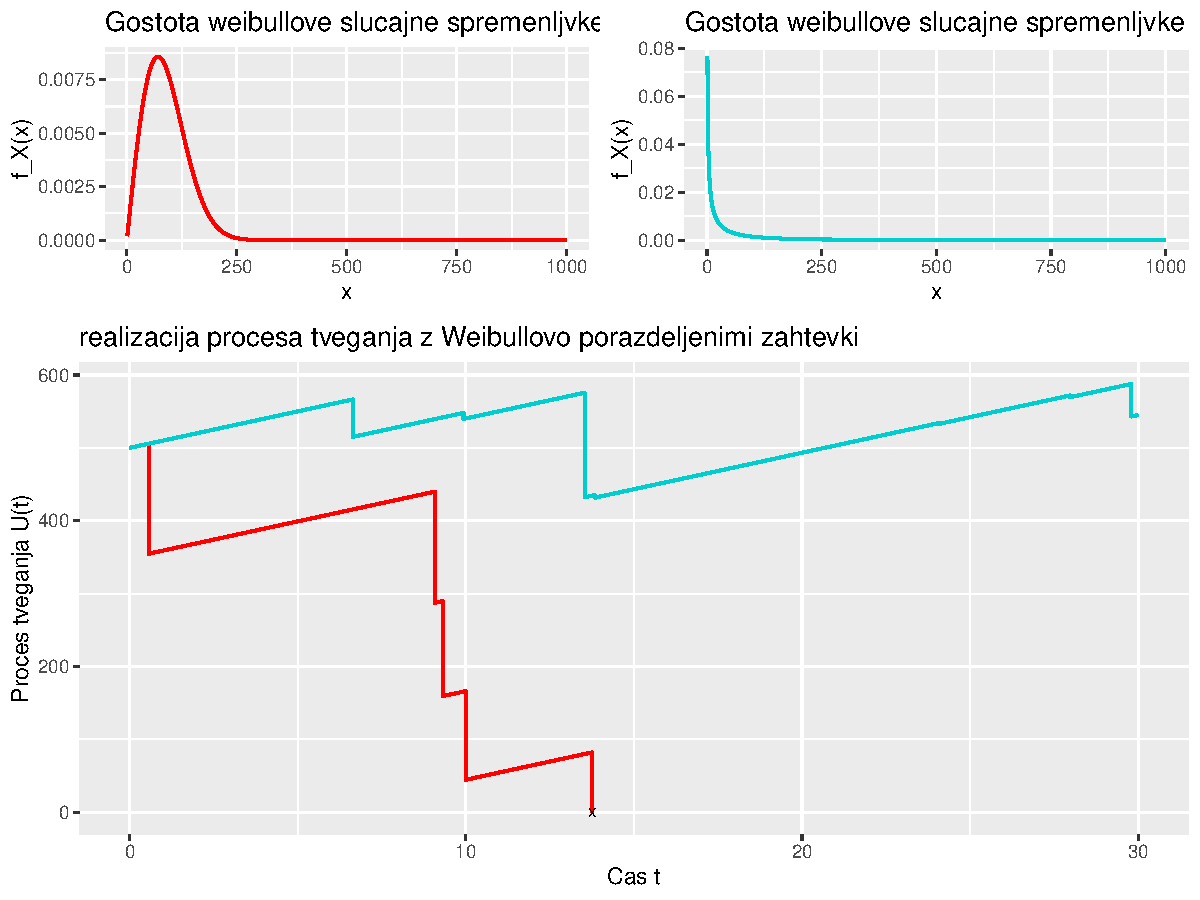
\includegraphics[width=\textwidth]{
    %            C:/Users/38651/OneDrive - Univerza v Ljubljani/Desktop/Diploma/Diplomski-seminar/GraphsAndPhotos/slika2.pdf
    %            }
    %        \caption{Histograma zahtevkov med 1.1.2015 in 1.3.2015}
    %        \label{fig:slika3}
    %    \end{figure}
%
    %    \begin{figure}[H]
    %        \centering
    %        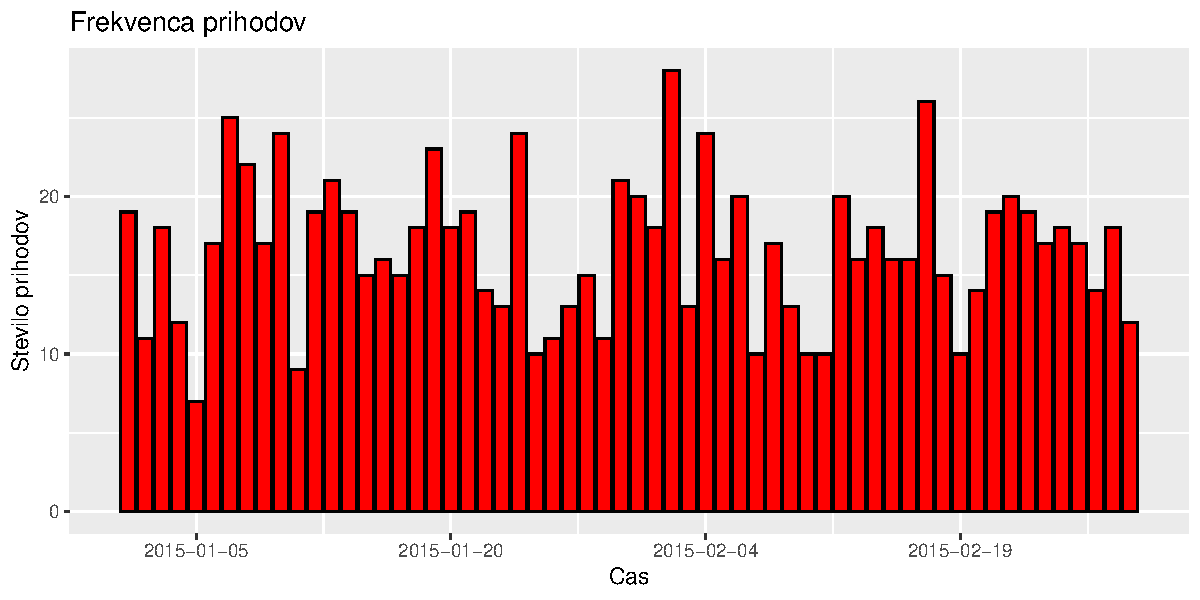
\includegraphics[width=\textwidth]{
    %            C:/Users/38651/OneDrive - Univerza v Ljubljani/Desktop/Diploma/Diplomski-seminar/GraphsAndPhotos/slika3.pdf
    %            }
    %        \caption{Stevilo prihodov zahtevkov na posamezen dan med 1.1.2015 in 1.3.2015}
    %        \label{fig:slika4}
    %    \end{figure}

        
        





\pagebreak

\section{Priloga}
    Dostavek je namenjen predvsem za dodatne definicije in trditve, ki so bile izpu"scene v glavnem
    za namene preglednosti besedila. V primeru, da bralec potrebuje osve"ziti dolo"cene pojme, 
    jih ve"cino lahko najde v tem razdelku.
    \begin{definicija}
        Naj bo $X$ slu"cajna spremenljivka. Potem so za $u\in\R$ njena \textit{rodovna funkcija}, 
        \textit{momentno rodovna funkcija} in \textit{karakteristi"cna funkcija} definirane 
        kot 
        \begin{equation*}
            G_X(u) = \E\left[u^X\right], \quad M_X(u) = \E\left[e^{uX}\right], \quad \varphi_X(u) = \E\left[e^{iuX}\right],
        \end{equation*}
        "ce upanja obstajajo.
        \label{def:rodovneFunkcije}
    \end{definicija}

    \begin{definicija}
        Slu"cajna spremenljivka $X$ ima \textit{Weibullovo porazdelitev} s parametri $a, b > 0$, 
        "ce ima njena porazdelitev obliko 
        \begin{equation*}
            F_X(x) = 1 - e^{-\left(\tfrac{x}{b}\right)^a} \quad \text{za} \ x\geq 0
        \end{equation*}
        in gostota obliko
        \begin{equation*}
            f_X(x) = \left(\frac{a}{b}\right)\left(\frac{x}{b}\right)^{a-1}e^{-\left(\tfrac{x}{b}\right)^a} \quad \text{za} \ x\geq 0.
        \end{equation*}
        \label{def:WeibullovaPorazdelitev}
    \end{definicija}

    \begin{trditev}
        Naj bo $X$ nenegativna slu"cajna spremenljivka na verjetnostnem prostoru $(\Omega, \mathcal{F}, \Prob)$, 
        ki ima prvi moment. Potem velja 
        \begin{equation*}
            \E\left[X\right] = \int_{(0, \infty)}\bigl(1 - F_X(x)\bigr)dx.
        \end{equation*}
        \label{trd:PricakovanaVrednostZPrezivetveno}
    \end{trditev}

    \begin{proof}
        $X$ lahko zapi"semo kot 
        \begin{equation*}
            X = \int_{(0, \infty)}\mathbbm{1}_{\{x < X\}}dx = \int_{(0, \infty)}\mathbbm{1}_{\{X < x\}}dx.
        \end{equation*}
        "Ce sedaj uporabimo fubinijev izrek dobimo
        \begin{align*}
            \E\left[X\right] &= \E\left[\int_{(0, \infty)}\mathbbm{1}_{\{X < x\}}dx\right] \\
                             &= \int_{(0, \infty)}\E\left[\mathbbm{1}_{\{X < x\}}\right]dx \\
                             &= \int_{(0, \infty)}\bigl(1 - \Prob\left(X > x\right)\bigr)dx \\
        \end{align*}
    \end{proof}

    \begin{trditev}(Neenakost Markova)
        \label{trd:neenakostMarkova}
        Naj bo $X$ nenegativna slu"cajna spremenljivka.
        Potem za  $x>0$ velja
        \begin{equation*}
            \Prob\left(X > x\right) \leq \frac{\E\left[X\right]}{x}.
        \end{equation*}
    \end{trditev}

    \begin{proof}
        Naj bo $x > 0$. Velja
        \begin{equation*}
            x\mathbbm{1}_{\{X > x\}} \leq X \iff x\Prob\left(X > x\right) \leq \E\left[X\right].
        \end{equation*}
    \end{proof}

    \begin{izrek}(Krepki zakon velikih "stevil)
        Naj bo $(X_n)_{n\in\N}$ zaporedje neodvisnih enako porazdeljenih
        slu"cajnih spremenljivk na verjetnostnem prostoru $(\Omega, \mathcal{F}, \Prob)$
         s pri"cakovano vrendostjo $\E\left[X_i\right] = \mu <\infty$. Potem velja
        \begin{equation*}
            \frac{X_1 + X_2 + \cdots X_n}{n}\xrightarrow[n\to\infty]{s.g.} \mu.
        \end{equation*}
        \label{izr:KrepkiZakonVelikihStevil}
    \end{izrek}

    \begin{proof}
        Dokaz izreka lahko bralec najde v \cite{7}.
    \end{proof}

    \begin{izrek}(Lévijev izrek o kontinuiteti)
        Naj bo $(X_n)_{n\in\N}$ zaporedje slu"cajnih spremenljivk (ne nujno na istem verjetnostnem prostoru)
        in $X$ "se ena slu"cajna spremenljivka. Potem za vsak $u\in\R$ velja
        \begin{equation*}
            \varphi_{X_n}(u) \xrightarrow{n\to\infty} \varphi_X(u) 
        \end{equation*}
        natanko tedaj, ko velja
        \begin{equation*}
            X_n \xrightarrow[n\to\infty]{d} X.
        \end{equation*}
        \label{izr:LevijevIzrek}
    \end{izrek}

    \begin{proof}
        Dokaz izreka lahko bralec najde v \cite{7}.
    \end{proof}

    \begin{izrek}(Lebesgueov izrek o monotoni konvergenci)
        Naj bo $X_1, X_2, \dots $ zaporedje nenegativnih slu"cajnih spremenljivk na 
        verjetnostnem prostoru $(\Omega, \mathcal{F}, \Prob)$ in naj bo $X:= \lim_{n\to\infty}X_n$ 
        njihova limita. Naj za vsak $\omega \in \Omega$
        velja $X_1(\omega) \leq X_2(\omega) \leq \dots$ Potem velja 
        \begin{equation*}
            \lim_{n\to\infty}\E\left[X_n\right] = \E\left[\lim_{n\to\infty}X_n\right] = \E\left[X\right].
        \end{equation*}
        \label{izr:monotonaKonvergenca}
    \end{izrek}

    \begin{proof}
        Dokaz izreka lahko bralec najde v \cite{7}.
    \end{proof}  

    \begin{izrek}(Tonellijev izrek)
        Naj bosta $X$ in $Y$ slu"cajni spremenljivki definirani vsaka na svojem verjentnostnem prostoru
        in naj imata vsaka svojo gostoto $f_X$ in $f_Y$ glede na Lebesgueovo mero.
        Potem velja
        \begin{equation*}
            \int_{\R^2}f_{X, Y}(x, y)\mathcal{L}^2(dx, dy) 
            = \int_{\R}\left(\int_{\R}f_{X, Y}(x, y)dx\right)dy = \int_{\R}\left(\int_{\R}f_{X, Y}(x, y)dy\right)dx.
        \end{equation*}
        \label{izr:TonellijevIzrek}
    \end{izrek}

    \begin{proof}
        Dokaz izreka lahko bralec najde v \cite{7}.
    \end{proof} 

    \begin{izrek}(Izrek o enoli"cnosti)
        One to one correspondence betwwen characteristic functions and distributions.
    \end{izrek}

    \begin{definicija}
        Naj bo $X$ nenegativna slu"cajna spremenljivka in $F_X$ njena porazdelitvena funkcija. 
        Potem za $u\in\R$ \textit{Laplace-Stiltjesovo transformacijo} porazdelitve $F_X$ definiramo kot
        \begin{equation*}
            \hat{F}_X(u) = \int_{[0, \infty)}e^{-ux}dF_X(x).
        \end{equation*}
        \label{def:LaplaceStiltjesovaTransformacija}
    \end{definicija}

    \begin{definicija}
        Naj bo $F$ porazdelitvena funckija neke nenegativne slu"cajne spremenljivke s prvim 
        momentom. Potem je 
        \begin{align*}
            \overline{F}(x) = \frac{1}{\mathbb{E}[X]} \int_0^x (1 - F(t)) \, dt
        \end{align*}
        \textit{porazdelitev integrarnega repa F}.
        \label{def:porazdelitevintegriranegaRepa}
    \end{definicija}

    \begin{definicija}
        \textit{Prenovitveni proces} na verjentostnem protoru $(\Omega, \mathcal{F}, \Prob)$ je slu"cajni 
        proces
        karatkteriziran z zaporedjem neodvisnih enako porazdeljenih medprihodnih "casov $(T_n)_{n\in\N}$, 
        ki zavzamejo vrednosti v $\R^+\cup\{\infty\}$ in je podan z zvezo 
        \begin{equation*}
            N_t = \sum_{n=1}^{\infty}\mathbbm{1}_{\{S_n\leq t\}},
        \end{equation*}
        kjer je $S_n = T_1 + T_2 + \cdots + T_n$ "cas $n$-tega prihoda. Pripadajo"co 
        \textit{prenovitveno mero} prenovitvenega procesa definiramo kot $M(t) = \E\left[N_t\right]$ za 
        $t > 0$.
        \label{def:PrenovitveniProces}
    \end{definicija}

    \begin{definicija}
        \textit{Prenovitvena ena"cba} je ena"cba oblike 
        \begin{equation*}
            f(t) = g(t) + \int_{[0, t]}f(t - s)dF(s), \quad t\geq 0,
        \end{equation*}
        kjer sta neznana funkcija $f$ in znana funckija $g$ definirani na $\R^+$ in $F$ je 
        porazdelitvna funkcija neke pozitivne slu"cajne spremenljivke $X$. Prenovitveno ena"cbo predstavimo
        s parom $(g, F)$.
        \label{def:prenovitvenaEnacba}
    \end{definicija}

    \begin{definicija}
        Za nenegativno merljivo funkcijo \( f : [0, \infty) \to [0, \infty) \) pravimo, da je \textit{direktno 
        Riemannovo integrabilna} (d.R.i.), če za vsak $\delta > 0$ velja
        \begin{equation*}
            \sum_{k \geq 0} \left( \sup_{t \in [k\delta, (k+1)\delta)} f(t) \right) < \infty \quad \text{in}
        \end{equation*}
        \begin{equation*}
             \lim_{\delta \downarrow 0} \delta \sum_{k \geq 0} \left( \sup_{t \in [k\delta, (k+1)\delta)} f(t) \right) = \lim_{\delta \downarrow 0} \delta \sum_{k \geq 0} \left( \inf_{t \in [k\delta, (k+1)\delta)} f(t) \right).
        \end{equation*}
        Če \(f\) zadošča navedenima zahtevama, potem je limita v drugi zahtevi točno vrednost direktnega Riemannovega integrala
        \[
        \text{d.R.i.} \int_{0}^{\infty} f(t) \, dt.
        \]
        Funkcija \(f\) poljubnega predznaka je d.R.i., če sta le-taki \(f^+ = \max\{f, 0\}\) in \(f^- = \max\{-f, 0\}\), pri čemer je
        \[
        \text{d.R.i.} \int_{0}^{\infty} f(t) \, dt = \text{d.R.i.} \int_{0}^{\infty} f^+(t) \, dt - \text{d.R.i.} \int_{0}^{\infty} f^-(t) \, dt.
        \]
        \label{def:direktnaRieamnovaIntegrabilnost}
    \end{definicija}

    \begin{trditev}(Kriterij za direktno Riemannovo integrabilnost)
        Naj bo $f \geq 0$ nenara"scajo"ca funkcija. Potem je $f$ direktno Riemannovo integrabilna natanko tedaj, ko je
        posplo"seno Riemannovo integrabilna. Tedaj je njen direktni riemannov integral enak posplo"senemu.
        \label{trd:kriterijZaDirektnoRiemannovoIntegrabilnost}
    \end{trditev}

    \begin{proof}
        Dokaz izreka lahko bralec najde v \cite{8} na strani 235. 
    \end{proof} 

    \begin{izrek}(Smithov klju"cni prenovitveni izrek)
        "Ce je funkcija $g$ iz prenovitvene ena"cbe $(g, F)$ (definicja \ref{def:prenovitvenaEnacba})
        omejena na kon"cnih intervalih in $X$ ima prvi moment ter ni aritmeti"cna 
        $(\nexists a\in\R: \ \Prob\left(X \in \mathbb{Z} a\right) = 1)$, potem je
        \begin{equation*}
            f(t) = g(t) +  \int_{[0, t]}g(t - s)dM(s), \quad t\geq 0,
        \end{equation*}
        enoli"cna re"sitev te ena"cbe. $M(s)$ pa prenovitvena mera prenovitvenega procesa z medprihodno 
        porazdelitvijo $F$.
        "Ce je dodatno funkcija $g$ direktno Riemannovo integrabilna velja 
        \begin{equation*}
            \lim_{t\to\infty}f(t) = \frac{1}{\E\left[X\right]}\int_{(0, \infty)}g(t)dt.
        \end{equation*}
        \label{izr:Smith}
    \end{izrek}

    \begin{proof}
        Dokaz izreka lahko bralec najde v \cite{8} na strani 237. 
    \end{proof}

%-----------------------------------------KONEC VSEBINE--------------------------------------------%

\section*{Slovar strokovnih izrazov}

\geslo{trajektorija}{sample path}
%
%\geslo{}{}
%


% Literatura
\begin{thebibliography}{99}
\bibitem{1}S.E. Shreve, Stochastic Calculus for Finance II: Continuous-Time Models, Springer, (2004).
\bibitem{2}S.M. Ross, Stochatic Processes: Second Edition, Wiley, (1996).
\bibitem{3}P. Embrechts, C. Klüppelberg, T. Mikosch, Modelling Extremal Events: For Insurance and Finance, Springer, (1997).
\bibitem{4}T. Mikosch, Non-Life Insurance Mathematics: An Introduction with the Poisson Process, Second Edition, Springer, (2009).
\bibitem{5}M. Mandjes, O. Boxma, The Cramér--Lundberg model and its variants, Springer, (2023).
\bibitem{6}F. Spitzer, Principles of Random Walk. Second Edition, Springer, (1976).
\bibitem{7}B. Fristedt, L. Gray, A Modern Approach to Probability Theory, Springer, (1996).
\bibitem{8}S.I. Resnick, Adventures in Stochastic Processes, Birkhäuser, (1992).
\end{thebibliography}

\end{document}